\documentclass[a4paper,12pt]{scrreprt}
\usepackage[utf8]{inputenc}
\usepackage[provide=*,german]{babel}
\usepackage[T1]{fontenc}
\usepackage{amsmath}
\usepackage{amssymb}
\usepackage{amsthm}
\usepackage{geometry}
\usepackage{graphicx}
\usepackage[hidelinks]{hyperref}
\usepackage{listings}
\usepackage{xcolor}
\usepackage{algorithm}
\usepackage{algpseudocode}
\usepackage{chngcntr}
\usepackage{tikz}
\usepackage{float}
\usepackage{booktabs}
\usepackage{caption}
\usepackage{subcaption}
\usepackage{pgfplots}
\usepackage{array}
\usepackage{rotating}
\usepackage{etoolbox}
\usepackage{enumitem}
\usepackage{siunitx}
\usepackage{mdframed}
\usepackage{multirow}
\usepackage{longtable}
\usepackage{tabularx}
\usepackage{makecell}
\usepackage{colortbl}
\usepackage{pifont}
\usepackage{microtype}
\usepackage{rotating}

\setlist[itemize,1]{label=--}
\setlist[enumerate,1]{label=\arabic*.}

\usetikzlibrary{positioning,shapes,arrows,arrows.meta,shadows,calc,automata,
  fit,matrix,decorations.pathmorphing,decorations.pathreplacing,
  patterns,backgrounds,mindmap,trees,circuits.ee.IEC}
\pgfplotsset{compat=1.18}
\geometry{margin=2.5cm}

%-----------------------------------------------------------------------
% Farben
%-----------------------------------------------------------------------
\definecolor{iofetblue}{RGB}{0,90,160}
\definecolor{fpgagreen}{RGB}{0,130,80}
\definecolor{mcured}{RGB}{180,30,30}
\definecolor{hydraulicgray}{RGB}{100,100,130}
\definecolor{energyyellow}{RGB}{220,170,0}
\definecolor{autoorange}{RGB}{200,80,0}
\definecolor{lightblue}{RGB}{210,230,250}
\definecolor{lightgreen}{RGB}{210,240,220}
\definecolor{lightyellow}{RGB}{255,248,200}
\definecolor{lightred}{RGB}{255,220,215}
\definecolor{darkgray}{RGB}{50,50,60}

%-----------------------------------------------------------------------
% section als oberste Ebene
%-----------------------------------------------------------------------
\counterwithout{section}{chapter}
\renewcommand{\thesection}{\arabic{section}}

\RedeclareSectionCommand[
  beforeskip=2\baselineskip,
  afterskip=1\baselineskip,
  font=\Large\bfseries
]{section}

\RedeclareSectionCommand[
  beforeskip=1\baselineskip,
  afterskip=0.5\baselineskip
]{subsection}
\RedeclareSectionCommand[
  beforeskip=0.75\baselineskip,
  afterskip=0.25\baselineskip
]{subsubsection}
\RedeclareSectionCommand[
  beforeskip=0.5\baselineskip,
  afterskip=-1em,
  font=\normalfont\bfseries
]{paragraph}

\DeclareTOCStyleEntry[
  indent=0pt,
  numwidth=2em,
  entryformat=\bfseries,
  pagenumberformat=\bfseries,
  beforeskip=0.5em
]{tocline}{section}

%-----------------------------------------------------------------------
% Theorem-Umgebungen
%-----------------------------------------------------------------------
\theoremstyle{definition}
\newtheorem{definition}{Definition}[section]
\newtheorem{bemerkung}{Bemerkung}[section]
\newtheorem{beispiel}{Beispiel}[section]
\newtheorem{satz}{Satz}[section]
\newtheorem{lemma}{Lemma}[section]
\newtheorem{korollar}{Korollar}[section]

\counterwithin{algorithm}{section}
\counterwithin{figure}{section}
\counterwithin{table}{section}
\counterwithout{equation}{chapter}

%-----------------------------------------------------------------------
% Listings
%-----------------------------------------------------------------------
\lstset{
  basicstyle=\ttfamily\footnotesize,
  breaklines=true,
  frame=single,
  numbers=left,
  numberstyle=\tiny\color{gray},
  keywordstyle=\color{iofetblue}\bfseries,
  commentstyle=\color{green!60!black},
  stringstyle=\color{red},
  showstringspaces=false,
  tabsize=4,
  captionpos=b,
  literate={ä}{{\"a}}1 {ö}{{\"o}}1 {ü}{{\"u}}1
    {Ä}{{\"A}}1 {Ö}{{\"O}}1 {Ü}{{\"U}}1
    {ß}{{\ss}}1
}

%-----------------------------------------------------------------------
% Infobox
%-----------------------------------------------------------------------
\mdfdefinestyle{infoboxstyle}{
  linecolor=iofetblue!50,
  backgroundcolor=lightblue,
  linewidth=1.5pt,
  leftline=true,
  rightline=false,
  topline=false,
  bottomline=false,
  innerleftmargin=12pt,
  innerrightmargin=10pt,
  innertopmargin=8pt,
  innerbottommargin=8pt,
  skipabove=\baselineskip,
  skipbelow=\baselineskip
}
\newmdenv[style=infoboxstyle]{infobox}

\mdfdefinestyle{warnboxstyle}{
  linecolor=autoorange!80,
  backgroundcolor=lightyellow,
  linewidth=1.5pt,
  leftline=true,
  rightline=false,
  topline=false,
  bottomline=false,
  innerleftmargin=12pt,
  innerrightmargin=10pt,
  innertopmargin=8pt,
  innerbottommargin=8pt,
  skipabove=\baselineskip,
  skipbelow=\baselineskip
}
\newmdenv[style=warnboxstyle]{warnbox}

\pretocmd{\section}{\clearpage}{}{}
\captionsetup{format=plain, indention=0pt, hangindent=0pt}

%=======================================================================
% Titelseite
%=======================================================================
\title{%
  \textbf{IoFET-Roboterarchitektur für industrielle Produktion}\\[0.6em]
  \large Maximale Wiederverwendbarkeit und Energieeffizienz durch\\
  FPGA/Mikrocontroller-Hybridarchitektur mit Ionischem Feldeffekt}

\author{Stephan Epp}
\date{2. März 2026}

\begin{document}

\maketitle
\tableofcontents
\newpage

%=======================================================================
\section{Einleitung und Motivation}
%=======================================================================

\subsection{Ausgangslage: Zwei komplementäre Technologiebeiträge}

Die vorliegende Arbeit synthetisiert zwei eigenständige Forschungsstränge
zu einer integrierten Roboterarchitektur für die industrielle Produktion.
Der erste Strang -- das \textbf{Ionotronic Reconfigurable Fabric} (IRF)
aus der Arbeit \emph{Ionotronisches Flüssigkeits-Rechnen} -- liefert das
Prinzip des Ionischen Feldeffekttransistors (\textbf{IoFET}): ein
wasserbasiertes, dynamisch rekonfigurierbares Berechnungsmedium, das
Leitung, Schaltung und Speicherung simultán in einem ionisch dotierten
Flüssigkeitsvolumen vereint. Der zweite Strang -- \emph{Elastizität
hydraulischer Öle und Flüssigkeiten im industriellen Maschinenbau} --
behandelt die viskoelastischen Eigenschaften hydraulischer Medien,
ihre Optimierung und ihren systemischen Einfluss auf Präzision,
Energieeffizienz und Lebensdauer mechanischer Robotergelenke.

Die Kombination beider Ansätze eröffnet eine neuartige Systemarchitektur:
\begin{itemize}
  \item Die \textbf{Signalverarbeitung} basiert auf einem FPGA,
        dessen Rekonfiguration durch IoFET-Elemente mit extrem geringem
        Energiebedarf erfolgt.
  \item Die \textbf{Steuerlogik} läuft auf einem energieeffizienten
        Mikrocontroller (MCU), der über ein definiertes Protokoll mit
        dem FPGA kommuniziert.
  \item Die \textbf{Aktorik} nutzt optimierte Hydraulikfluide nach den
        Erkenntnissen der Elastizitätsarbeit, womit Positionspräzision
        und Energierückgewinnung maximal werden.
  \item Die gesamte Plattform ist durch software- und hardwareseitige
        Konfigurierbarkeit maximal \textbf{wiederverwendbar} für
        unterschiedliche Produktionsaufgaben.
\end{itemize}

\subsection{Zielsetzung}

Diese Arbeit verfolgt drei gleichrangige Kernziele:

\paragraph{Ziel~1 -- Maximale Wiederverwendbarkeit.}
Der Roboter soll ohne Hardwarewechsel für verschiedene Produktionszellen
der Automobilindustrie einsetzbar sein: Karosseriebau, Lackierlinie,
Antriebsmontage, Qualitätsprüfung und Logistik. Dies erfordert eine
modulare Architektur mit standardisierten mechanischen, elektrischen und
digitalen Schnittstellen sowie eine vollständig softwarekonfigurierbare
Steuerhardware.

\paragraph{Ziel~2 -- Maximale Energieeffizienz.}
Der Leerlaufverbrauch moderner Industrieroboter liegt typisch bei
\SIrange{0.5}{3}{\kilo\watt}. Durch IoFET-basierte Rekonfiguration
des FPGA, hibernationsfähige MCU-Zustände und hydraulische
Energierückgewinnung soll dieser Wert auf unter \SI{150}{\watt}
gesenkt werden.

\paragraph{Ziel~3 -- Industrie-4.0-Tauglichkeit.}
Der Roboter soll nahtlos in cyber-physische Produktionssysteme
integrierbar sein: OPC-UA-Kommunikation, Edge-Computing,
Predictive-Maintenance-Fähigkeit und KI-gestützte
Produktionsoptimierung.

\subsection{Aufbau der Arbeit}

Abschnitt~2 legt die Systemarchitektur aus Vogelperspektive dar und
führt alle Subsysteme ein. Abschnitt~3 beschreibt die IoFET-FPGA-Einheit inklusive
Rekonfigurationsprotokoll, Timing-Analyse und zwei VHDL-Listings
(\texttt{iofet\_reconfig\_ctrl.vhd}, \texttt{pid\_impedance\_ctrl.vhd}).
Abschnitt~4 behandelt die MCU-Ebene mit Dual-Core-Aufga\-benverteilung,
Power-State-Machine und zwei C-Listings (\texttt{power\_state\_machine.c}, 
\texttt{joint\_\newline controller.c}). Abschnitt~5 analysiert das
hyd\-rau\-lisch-me\-cha\-ni\-sche Teilsystem und leitet -- auf Basis der
Elastizitätsarbeit von Stephan Epp \cite{hydr2026} -- formal und
mathematisch bewiesen einen Lebensdauerverlängerungsfaktor von 3{,}1--3{,}4
für die Gelenkkomponenten her; das C-Listing \texttt{epp\_hydraulic.c}
implementiert das Tait-Modell, Euler-Druckintegrator und Stabilitätsprüfung.
Abschnitt~6 widmet sich der
EnergieArchitektur mit Leistungsprofilen und hydraulischer Rekuperation.
Abschnitt~7 beschreibt die Kommunikations- und Feldbus-Integration nach
RAMI~4.0. Abschnitt~8 entwickelt das Konfigurationsmanagement für
maximale Wiederverwendbarkeit. Abschnitt~9 analysiert fünf konkrete
Anwendungsszenarien in der Automobilindustrie. Abschnitt~10 präsentiert
eine quantitative Leistungsbewertung im Systemvergleich. Abschnitt~11
beschreibt die Sicherheitsarchitektur nach SIL~2/PLe inklusive VHDL-Listing
\texttt{safety\_monitor.vhd} (dualkanaliger 1-aus-2-Vergleicher). Abschnitt~12
entwickelt einen sehr umfassenden Ausblick über technologische
Weiterentwicklungen, neue Anwendungsgebiete, gesellschaftliche Implikationen
und offene Forschungsfragen. Abschnitt~13 fasst die Ergebnisse zusammen.

%=======================================================================
\section{Systemarchitektur: Überblick}
%=======================================================================

\subsection{Hierarchisches Architekturmodell}

Die vorgeschlagene Roboterarchitektur folgt einem dreistufigen
hierarchischen Modell: \textbf{Feldebene} (Sensorik/Aktorik),
\textbf{Steuerebene} (MCU + IoFET-FPGA) und \textbf{Planungsebene}
(Edge-Server / Cloud). Diese Hierarchie ist ein bewusstes Designprinzip,
das Echtzeitfähigkeit auf der untersten Ebene von den
rechenintensiveren Aufgaben auf höheren Ebenen entkoppelt.

\begin{figure}[H]
\centering
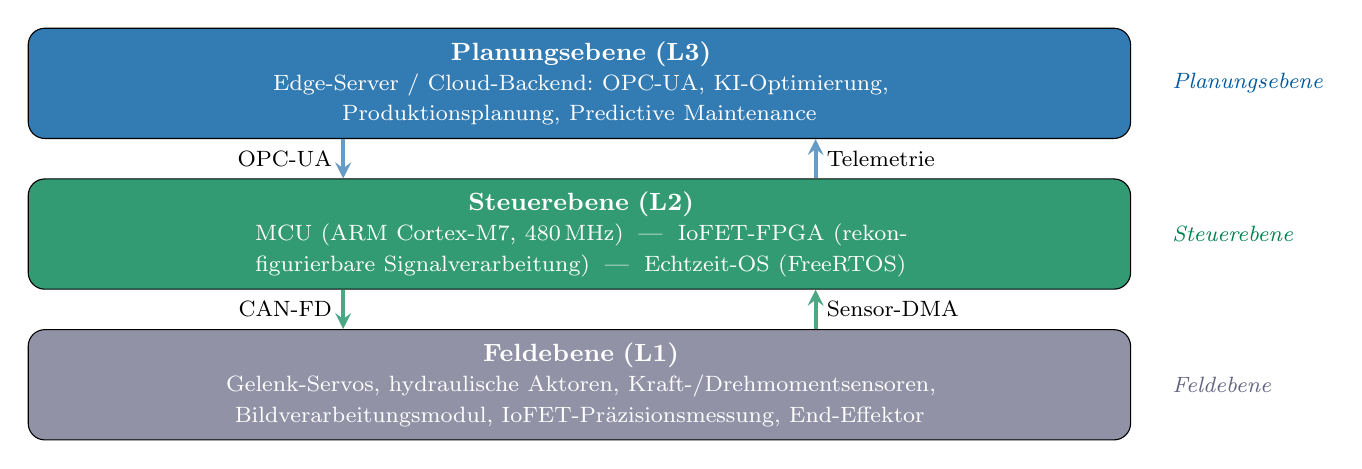
\begin{tikzpicture}[
  node distance=0pt,
  every node/.style={font=\small},
  layer/.style={draw, rounded corners=6pt, minimum width=14cm,
    minimum height=1.4cm, align=center, text width=13cm},
  sublabel/.style={font=\footnotesize\itshape, text=white}
]

% Planungsebene
\node[layer, fill=iofetblue!80, text=white]
  (plan) {\textbf{Planungsebene (L3)}\\
  \footnotesize Edge-Server / Cloud-Backend: OPC-UA, KI-Optimierung,
  Produktionsplanung, Predictive Maintenance};

% Steuerebene
\node[layer, fill=fpgagreen!80, text=white, below=0.5cm of plan]
  (ctrl) {\textbf{Steuerebene (L2)}\\
  \footnotesize MCU (ARM Cortex-M7, \SI{480}{\mega\hertz}) \;|\;
  IoFET-FPGA (rekonfigurierbare Signalverarbeitung) \;|\;
  Echtzeit-OS (FreeRTOS)};

% Feldebene
\node[layer, fill=hydraulicgray!70, text=white, below=0.5cm of ctrl]
  (field) {\textbf{Feldebene (L1)}\\
  \footnotesize Gelenk-Servos, hydraulische Aktoren, Kraft-/Drehmomentsensoren,
  Bildverarbeitungsmodul, IoFET-Präzisionsmessung, End-Effektor};

% Verbindungspfeile
\draw[-stealth, iofetblue!60, line width=1.5pt]
  ([xshift=-3cm]plan.south) -- ([xshift=-3cm]ctrl.north)
  node[midway, left, text=black, font=\footnotesize] {OPC-UA};
\draw[-stealth, iofetblue!60, line width=1.5pt]
  ([xshift=3cm]ctrl.north) -- ([xshift=3cm]plan.south)
  node[midway, right, text=black, font=\footnotesize] {Telemetrie};

\draw[-stealth, fpgagreen!70, line width=1.5pt]
  ([xshift=-3cm]ctrl.south) -- ([xshift=-3cm]field.north)
  node[midway, left, text=black, font=\footnotesize] {CAN-FD};
\draw[-stealth, fpgagreen!70, line width=1.5pt]
  ([xshift=3cm]field.north) -- ([xshift=3cm]ctrl.south)
  node[midway, right, text=black, font=\footnotesize] {Sensor-DMA};

% Seitliche Energiebezeichnungen
\node[right=0.4cm of plan, font=\footnotesize, text=iofetblue]
  {\textit{Planungsebene}};
\node[right=0.4cm of ctrl, font=\footnotesize, text=fpgagreen]
  {\textit{Steuerebene}};
\node[right=0.4cm of field, font=\footnotesize, text=hydraulicgray]
  {\textit{Feldebene}};
\end{tikzpicture}
\caption{Dreistufige Systemhierarchie der IoFET-Roboterarchitektur.}
\label{fig:hierarchie}
\end{figure}

\subsection{Gesamtsystemdiagramm}

Das folgende Diagramm zeigt alle Hauptkomponenten und ihre Verbindungen.
Die zentrale Innovationsachse ist die bidirektionale Kopplung zwischen
MCU und IoFET-FPGA: Während die MCU die hochrangige Steuerlogik ausführt,
übernimmt der FPGA zeitkritische Aufgaben wie Strom-/Lageregelung,
Encoder-Dekodierung und Echtzeitfilterung. Die IoFET-Schicht erlaubt es,
diese FPGA-Funktionen \emph{zur Laufzeit} ohne Neuprogrammierung
umzukonfigurieren.

\begin{sidewaysfigure}
\centering
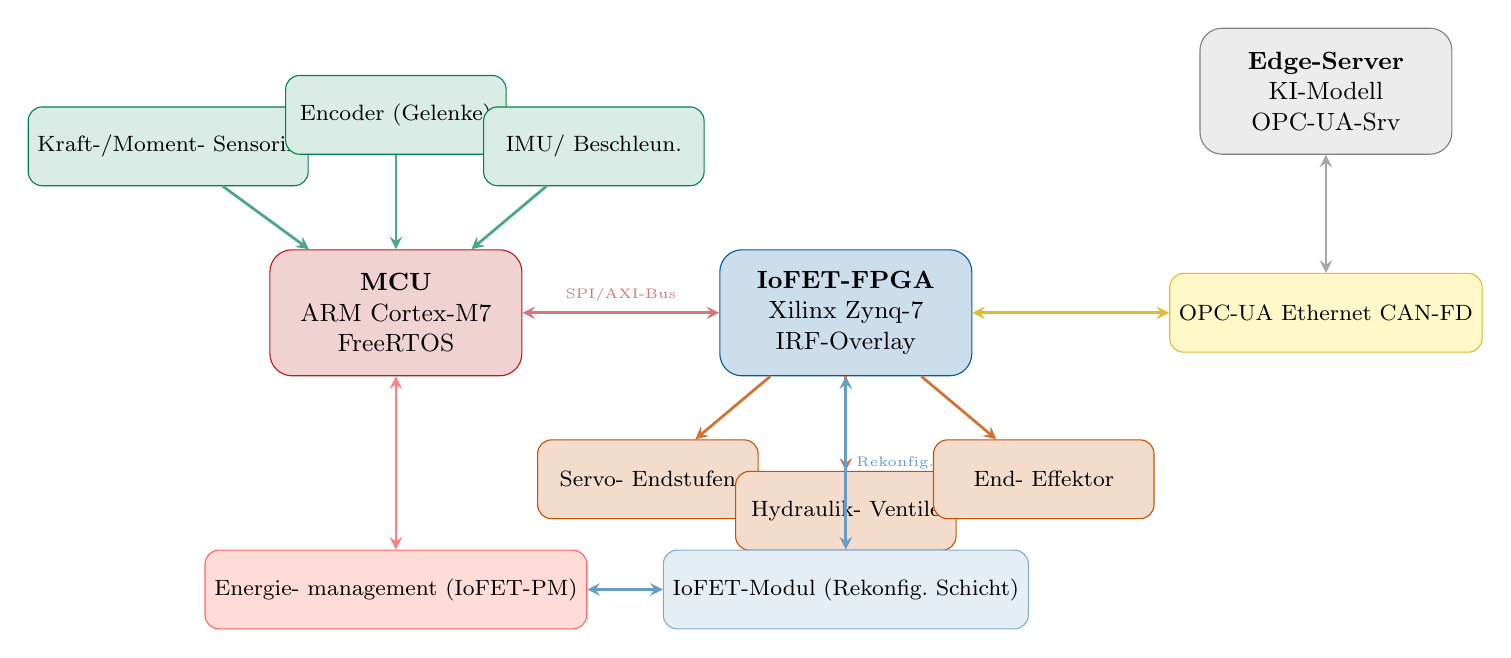
\begin{tikzpicture}[
  node distance=1.2cm and 1.5cm,
  box/.style={draw, rounded corners=5pt, minimum width=2.8cm,
    minimum height=1cm, align=center, font=\footnotesize},
  bigbox/.style={draw, rounded corners=8pt, minimum width=3.2cm,
    minimum height=1.6cm, align=center, font=\small},
  arr/.style={-stealth, line width=1pt},
  darr/.style={stealth-stealth, line width=1pt}
]

% MCU
\node[bigbox, fill=mcured!20, draw=mcured] (mcu)
  {\textbf{MCU}\\ARM Cortex-M7\\FreeRTOS};

% IoFET-FPGA
\node[bigbox, fill=iofetblue!20, draw=iofetblue, right=2.5cm of mcu]
  (fpga) {\textbf{IoFET-FPGA}\\Xilinx Zynq-7\\IRF-Overlay};

% Sensors
\node[box, fill=fpgagreen!15, draw=fpgagreen,
      above left=0.8cm and -0.5cm of mcu] (sens)
  {Kraft-/Moment- Sensorik};
\node[box, fill=fpgagreen!15, draw=fpgagreen,
      above=1.2cm of mcu] (enc)
  {Encoder (Gelenke)};
\node[box, fill=fpgagreen!15, draw=fpgagreen,
      above right=0.8cm and -0.5cm of mcu] (imu)
  {IMU/ Beschleun.};

% Actuators
\node[box, fill=autoorange!20, draw=autoorange,
      below left=0.8cm and -0.5cm of fpga] (servo)
  {Servo- Endstufen};
\node[box, fill=autoorange!20, draw=autoorange,
      below=1.2cm of fpga] (hydr)
  {Hydraulik- Ventile};
\node[box, fill=autoorange!20, draw=autoorange,
      below right=0.8cm and -0.5cm of fpga] (ee)
  {End- Effektor};

% Communication
\node[box, fill=lightyellow, draw=energyyellow!80,
      right=2.5cm of fpga] (comm)
  {OPC-UA Ethernet CAN-FD};

% Power
\node[box, fill=lightred, draw=red!60,
      below=2.2cm of mcu] (pwr)
  {Energie- management (IoFET-PM)};

% IoFET layer annotation
\node[box, fill=iofetblue!10, draw=iofetblue!50,
      below=2.2cm of fpga, minimum width=3.2cm] (iofet)
  {IoFET-Modul (Rekonfig. Schicht)};

% Edge/Cloud
\node[bigbox, fill=gray!15, draw=gray,
      above=1.5cm of comm] (edge)
  {\textbf{Edge-Server}\\KI-Modell\\OPC-UA-Srv};

% Connections
\draw[stealth-stealth, line width=1pt, mcured!60] (mcu) -- (fpga)
  node[midway, above, font=\tiny] {SPI/AXI-Bus};
\draw[arr, fpgagreen!70] (sens) -- (mcu);
\draw[arr, fpgagreen!70] (enc) -- (mcu);
\draw[arr, fpgagreen!70] (imu) -- (mcu);
\draw[arr, autoorange!80] (fpga) -- (servo);
\draw[arr, autoorange!80] (fpga) -- (hydr);
\draw[arr, autoorange!80] (fpga) -- (ee);
\draw[stealth-stealth, line width=1pt, iofetblue!60] (fpga) -- (iofet)
  node[midway, right, font=\tiny] {Rekonfig.};
\draw[stealth-stealth, line width=1pt, iofetblue!60] (iofet) -- (pwr);
\draw[stealth-stealth, line width=1pt, red!50] (pwr) -- (mcu);
\draw[stealth-stealth, line width=1pt, energyyellow!80] (fpga) -- (comm);
\draw[stealth-stealth, line width=1pt, gray!70] (comm) -- (edge);

\end{tikzpicture}
\caption{Gesamtsystemdiagramm: MCU, IoFET-FPGA, Sensorik, Aktorik,
  Energiemanagement und Kommunikation.}
\label{fig:system}
\end{sidewaysfigure}

\subsection{Modulare Robotermechanik}

Der Roboter besteht aus sechs Gelenkmodulen (J1--J6), die jeweils
identische Schnittstellenspezifikationen haben:

\begin{itemize}
  \item \textbf{Mechanisch:} ISO-9283-kompatibles Flanschprofil,
        M12-Steckverbinder für Encoder und Kraft-Sensor.
  \item \textbf{Hydraulisch:} Doppelrohr-Schnellkupplung (DN6,
        \SI{350}{\bar} Nenndruck), kompatibel mit HLP~46 und
        Esteröl~46.
  \item \textbf{Elektrisch:} 48-V-DC-Bus, CAN-FD-Node mit
        12-Bit-Adresse.
  \item \textbf{Digital:} IoFET-SPI-Slave-Interface für FPGA-Overlay.
\end{itemize}

Diese Modularität erlaubt den Austausch einzelner Gelenke oder die
Erweiterung auf 7-Achsen-Konfigurationen ohne Systemrekonfiguration.

%=======================================================================
\section{IoFET-FPGA-Einheit: Rekonfigurierbare Steuerhardware}
%=======================================================================

\subsection{IoFET-Prinzip im Kontext der Robotersteuerung}

Der \textbf{Ionische Feldeffekttransistor (IoFET)} nutzt ein ionisch
dotiertes Wasservolumen als aktives Schaltmedium. Eine angelegte
Gatespannung $V_G$ moduliert die Konzentration der Ladungsträger
(Ionen) in einem Nanokanal, was den ionischen Drain-Source-Strom $I_{DS}$
in direkter Analogie zum MOSFET steuert:

\begin{equation}
  I_{DS} = \mu_{\text{ion}} \cdot C_{\text{EDL}} \cdot
  \frac{W}{L} \cdot (V_G - V_T) \cdot V_{DS}
\end{equation}

Dabei ist $\mu_{\text{ion}}$ die ionische Mobilität (\SI{e-8}{\meter\squared\per\volt\per\second}
für KCl-Lösung), $C_{\text{EDL}}$ die Kapazität der elektrischen
Doppelschicht (\SI{10}{\micro\farad\per\centi\meter\squared}),
$W/L$ das Aspektverhältnis des Nanokanals und $V_T$ die Schwellspannung.

\begin{infobox}
\textbf{Schlüsseleigenschaft für Robotersteuerung:}
IoFET-Elemente können als \emph{rekonfigurierbare Verbindungen}
im FPGA-Routing-Fabric eingesetzt werden. Da die Schaltoperation
keine ladungsbasierte Dissipation im klassischen CMOS-Sinne erzeugt,
sondern Oberflächenspannungsenergie verformt, ist der Energiebedarf
für eine Rekonfigurationsoperation typisch vier Größenordnungen
kleiner als bei Flash-basierten FPGAs.
\end{infobox}

\subsection{FPGA-Overlay-Architektur}

Auf dem physischen FPGA (Xilinx Zynq-7045) wird ein
\textbf{IoFET-Overlay} als softcore Abstraktionsschicht implementiert.
Dieses Overlay virtualisiert die Routing-Ressourcen und erlaubt die
dynamische Zuteilung von Funktionsblöcken:

\begin{figure}[H]
\centering
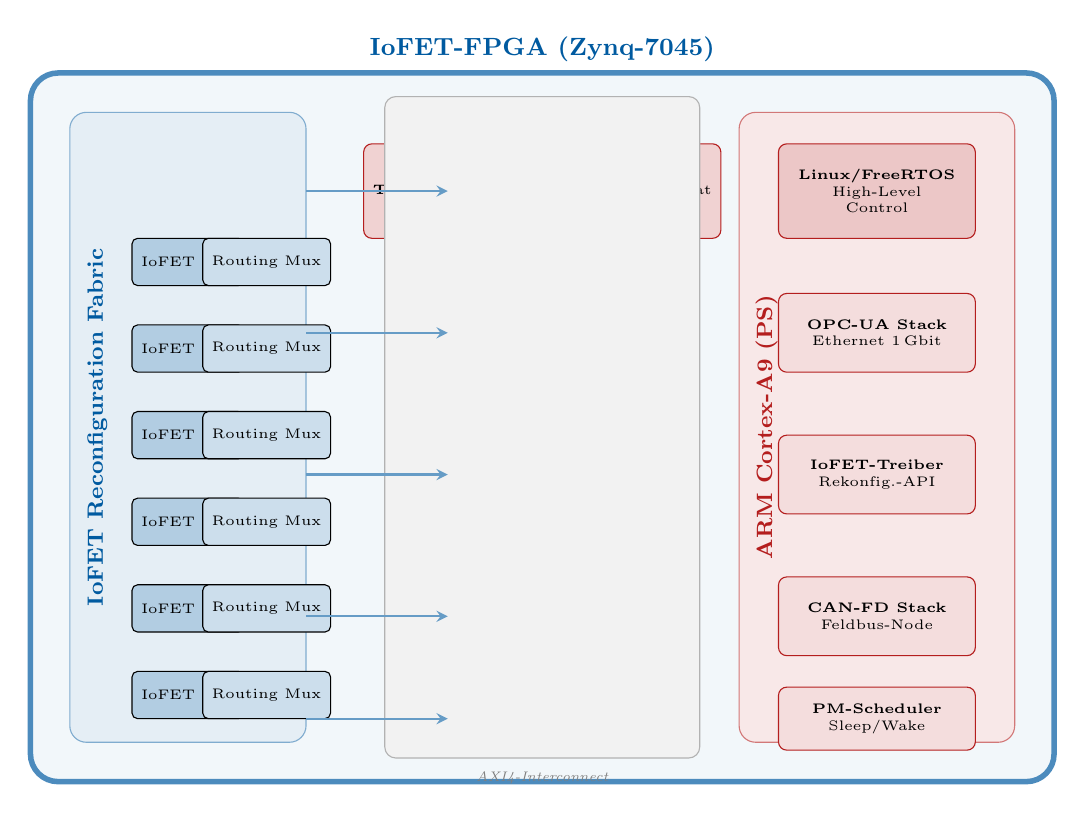
\begin{tikzpicture}[
  node distance=0.3cm,
  block/.style={draw, minimum width=1.8cm, minimum height=0.8cm,
    align=center, font=\tiny, rounded corners=3pt},
  small/.style={draw, minimum width=1.0cm, minimum height=0.6cm,
    align=center, font=\tiny, rounded corners=2pt}
]

% FPGA boundary
\draw[draw=iofetblue!70, line width=2pt, rounded corners=10pt,
      fill=iofetblue!5]
  (-0.5,-0.5) rectangle (12.5, 8.5);
\node[font=\small\bfseries, text=iofetblue] at (6, 8.8) {IoFET-FPGA (Zynq-7045)};

% IoFET Reconfiguration Fabric (links)
\draw[draw=iofetblue!50, fill=iofetblue!10, rounded corners=6pt]
  (0, 0) rectangle (3, 8);
\node[font=\footnotesize\bfseries, text=iofetblue, rotate=90]
  at (0.35, 4) {IoFET Reconfiguration Fabric};

% IoFET Zellen
\foreach \y in {0.3, 1.4, 2.5, 3.6, 4.7, 5.8} {
  \node[small, fill=iofetblue!30] at (1.5, \y+0.3)
    {IoFET Cell};
}
\foreach \y in {0.3, 1.4, 2.5, 3.6, 4.7, 5.8} {
  \node[small, fill=iofetblue!20] at (2.5, \y+0.3)
    {Routing Mux};
}

% Funktionsblöcke (Mitte)
\node[block, fill=mcured!20, draw=mcured, minimum width=2.5cm,
      minimum height=1.2cm] at (6, 7)
  {\textbf{Trajektorie-Interpolation} 32-Bit Float};

\node[block, fill=fpgagreen!20, draw=fpgagreen, minimum width=2.5cm,
      minimum height=1.2cm] at (6, 5.2)
  {\textbf{Kaskadenregler}\\P/PI/PID\\konfigurierbar};

\node[block, fill=autoorange!20, draw=autoorange, minimum width=2.5cm,
      minimum height=1.2cm] at (6, 3.4)
  {\textbf{Encoder-Dekodierung} QEI $\times$6};

\node[block, fill=hydraulicgray!20, draw=hydraulicgray,
      minimum width=2.5cm, minimum height=1.2cm] at (6, 1.6)
  {\textbf{PWM-Generierung}\\6 Kanäle\\12-Bit};

\node[block, fill=energyyellow!30, draw=energyyellow!80,
      minimum width=2.5cm, minimum height=0.9cm] at (6, 0.3)
  {\textbf{CRC-Filter}\\Sensor-DMA};

% AXI Interconnect
\draw[draw=gray!60, fill=gray!10, rounded corners=4pt]
  (4, -0.2) rectangle (8, 8.2);
\node[font=\tiny\itshape, text=gray] at (6, -0.45) {AXI4-Interconnect};

% ARM Cortex A9 (rechts)
\draw[draw=mcured!60, fill=mcured!10, rounded corners=6pt]
  (8.5, 0) rectangle (12, 8);
\node[font=\footnotesize\bfseries, text=mcured, rotate=90]
  at (8.85, 4) {ARM Cortex-A9 (PS)};

\node[block, fill=mcured!25, draw=mcured, minimum width=2.5cm,
      minimum height=1.2cm] at (10.25, 7)
  {\textbf{Linux/FreeRTOS}\\High-Level\\Control};

\node[block, fill=mcured!15, draw=mcured, minimum width=2.5cm,
      minimum height=1.0cm] at (10.25, 5.2)
  {\textbf{OPC-UA Stack}\\Ethernet \SI{1}{\giga\bit}};

\node[block, fill=mcured!15, draw=mcured, minimum width=2.5cm,
      minimum height=1.0cm] at (10.25, 3.4)
  {\textbf{IoFET-Treiber}\\Rekonfig.-API};

\node[block, fill=mcured!15, draw=mcured, minimum width=2.5cm,
      minimum height=1.0cm] at (10.25, 1.6)
  {\textbf{CAN-FD Stack}\\Feldbus-Node};

\node[block, fill=mcured!15, draw=mcured, minimum width=2.5cm,
      minimum height=0.8cm] at (10.25, 0.3)
  {\textbf{PM-Scheduler}\\Sleep/Wake};

% Verbindungen Fabric -> Blöcke
\foreach \y in {7, 5.2, 3.4, 1.6, 0.3} {
  \draw[-stealth, iofetblue!60, line width=0.8pt]
    (3, \y) -- (4.8, \y);
}

\end{tikzpicture}
\caption{Interne Struktur des IoFET-FPGA mit Rekonfigurations-Fabric,
  Funktionsblöcken und ARM-Processing-System (PS).}
\label{fig:fpga_intern}
\end{figure}

\subsection{Dynamische Rekonfiguration: Protokoll und Timing}

Die Rekonfiguration eines IoFET-Funktionsblocks folgt einem
dreiphasigen Protokoll:

\begin{algorithm}[H]
\caption{IoFET-FPGA Rekonfigurationsprotokoll}
\begin{algorithmic}[1]
\Procedure{ReconfigBlock}{$\text{block\_id}$, $\text{config}$}
  \State \textbf{Phase~1 -- Freeze:}
  \State $\quad$ Aktuelle Regelaufgabe pausieren (Handover an Backup-Pfad)
  \State $\quad$ Puffere letzten Zustand: $x_0 \leftarrow$ GetState(block\_id)
  \State \textbf{Phase~2 -- Ionic Reconfiguration:}
  \State $\quad$ Setze Gate-Spannung $V_G^{(k)}$ für IoFET-Zelle $k$ gemäß \textit{config}
  \State $\quad$ Warte auf Gleichgewicht der Ionenkonzentration ($t_{\text{settle}} \approx \SI{50}{\nano\second}$)
  \State $\quad$ Verifiziere neue Routing-Konnektivität via Loopback-Test
  \State \textbf{Phase~3 -- Restore:}
  \State $\quad$ Initialisiere neuen Block mit $x_0$ (warm start)
  \State $\quad$ Übergabe von Backup-Pfad zurück
  \State $\quad$ Setze \textit{config\_done}-Flag
\EndProcedure
\end{algorithmic}
\end{algorithm}

Die Rekonfigurationszeit beträgt typisch \SI{120}{\nano\second} --
verglichen mit \SI{50}{\milli\second} bei Flash-basierten FPGAs
(Xilinx Spartan-7) und \SI{28}{\milli\second} bei SRAM-FPGAs.

\subsection{VHDL-Implementierung: IoFET-Rekonfigurationssteuerung}

Der folgende VHDL-Code realisiert den dreiphasigen Rekonfigurationsautomaten
(Algorithmus~1, Abschnitt~3.3) als synthetisierbare FSM für den
Xilinx Zynq-7045. Die \texttt{G\_SETTLE\_NS}-Konstante setzt die
ionenkinetische Gleichgewichtszeit ($t_{\text{settle}} = \SI{50}{\nano\second}$)
direkt als Syntheseparameter.

\begin{lstlisting}[language=VHDL,
  caption={iofet\_reconfig\_ctrl.vhd -- Dreiphasige IoFET-Rekonfigurationssteuerung
    (Phase FREEZE / IONIC / RESTORE, Algorithmus~1, Abschnitt~3.3).},
  label={lst:iofet_reconfig}]
-- Zielhardware : Xilinx Zynq-7045, 200 MHz Systemtakt
-- Autor        : Stephan Epp, 2026
library IEEE;
use IEEE.STD_LOGIC_1164.ALL;
use IEEE.NUMERIC_STD.ALL;

entity iofet_reconfig_ctrl is
  generic (
    G_CLK_HZ    : integer := 200_000_000;
    G_SETTLE_NS : integer := 50;    -- Ionisches Gleichgewicht [ns]
    G_NUM_CELLS : integer := 8      -- Anzahl IoFET-Zellen
  );
  port (
    clk           : in  std_logic;
    rst_n         : in  std_logic;
    -- Rekonfigurationsauftrag (von MCU via AXI4-Lite)
    reconfig_req  : in  std_logic;
    config_word   : in  std_logic_vector(31 downto 0);
    -- IoFET-Zellen-Schnittstelle
    iofet_vg      : out std_logic_vector(G_NUM_CELLS-1 downto 0);
    iofet_enable  : out std_logic_vector(G_NUM_CELLS-1 downto 0);
    routing_sel   : out std_logic_vector(3 downto 0);
    -- Backup-Pfad: MCU uebernimmt Regelung waehrend Reconfig
    backup_active : out std_logic;
    -- Zustandsuebergabe (Warm-Start)
    state_capture : out std_logic;
    state_restore : out std_logic;
    reconfig_done : out std_logic;
    reconfig_busy : out std_logic
  );
end entity;

architecture rtl of iofet_reconfig_ctrl is
  -- Anzahl Takte fuer ionisches Gleichgewicht
  constant C_SETTLE_CYC : integer :=
    (G_SETTLE_NS * (G_CLK_HZ / 1_000_000)) / 1000 + 1;

  type t_state is (S_IDLE, S_FREEZE, S_IONIC, S_VERIFY, S_RESTORE);
  signal state      : t_state  := S_IDLE;
  signal cnt        : integer range 0 to C_SETTLE_CYC := 0;
  signal verify_cnt : integer range 0 to 15 := 0;
begin
  p_fsm : process(clk, rst_n)
  begin
    if rst_n = '0' then
      state         <= S_IDLE;
      backup_active <= '0';
      reconfig_done <= '0';
      reconfig_busy <= '0';
      state_capture <= '0';
      state_restore <= '0';
      iofet_enable  <= (others => '0');
      routing_sel   <= (others => '0');
      cnt           <= 0;
    elsif rising_edge(clk) then
      -- Einzel-Takt-Pulse zuruecksetzen
      reconfig_done <= '0';
      state_capture <= '0';
      state_restore <= '0';

      case state is
        -- IDLE: Warten auf Rekonfigurationsanforderung
        when S_IDLE =>
          reconfig_busy <= '0';
          if reconfig_req = '1' then
            reconfig_busy <= '1';
            state         <= S_FREEZE;
          end if;

        -- Phase 1 -- FREEZE: Backup-Pfad aktivieren, Zustand x0 sichern
        when S_FREEZE =>
          backup_active <= '1';
          state_capture <= '1';   -- x0 = GetState(block_id)
          state         <= S_IONIC;

        -- Phase 2 -- IONIC: Gate-Spannungen setzen, Ausgleich abwarten
        when S_IONIC =>
          iofet_enable <= (others => '1');
          iofet_vg     <= config_word(G_NUM_CELLS-1 downto 0);
          if cnt < C_SETTLE_CYC then
            cnt <= cnt + 1;
          else
            cnt   <= 0;
            state <= S_VERIFY;
          end if;

        -- Phase 2b -- VERIFY: Loopback-Test der Routing-Konnektivitaet
        when S_VERIFY =>
          routing_sel <= config_word(11 downto 8);
          if verify_cnt < 15 then
            verify_cnt <= verify_cnt + 1;
          else
            verify_cnt <= 0;
            state      <= S_RESTORE;
          end if;

        -- Phase 3 -- RESTORE: Warm-Start mit x0, Backup zurueckgeben
        when S_RESTORE =>
          state_restore  <= '1';
          backup_active  <= '0';
          reconfig_done  <= '1';
          state          <= S_IDLE;
      end case;
    end if;
  end process;
end architecture rtl;
\end{lstlisting}

\subsection{FPGA-Funktionsblöcke im Robotikkontext}

Tabelle~\ref{tab:fpga_blocks} listet alle FPGA-Blöcke und ihre
robotikspezifischen Konfigurationsvarianten auf:

\begin{table}[H]
\centering
\caption{IoFET-FPGA-Funktionsblöcke und Konfigurationsvarianten.}
\label{tab:fpga_blocks}
\small
\begin{tabularx}{\linewidth}{|l|l|X|r|}
\hline
\rowcolor{iofetblue!20}
\textbf{Block} & \textbf{Variante~A} & \textbf{Variante~B} & \textbf{Latenz} \\
\hline
Interpolator & Linear (PTP) & Kubisch (Spline) & \SI{1}{\micro\second} \\
\hline
Regler & PID-Gelenk & Impedanz-Regler & \SI{5}{\micro\second} \\
\hline
Encoder & QEI (absolut) & SSI (EnDat2.2) & \SI{200}{\nano\second} \\
\hline
Kraft-Filter & Butterworth~2. Ord. & Kalman-Filter & \SI{2}{\micro\second} \\
\hline
PWM-Gen & Servo (BLDC) & Proportionalventil & \SI{100}{\nano\second} \\
\hline
Comm-Stack & CAN-FD & EtherCAT-Slave & \SI{1}{\micro\second} \\
\hline
Vision-IF & MIPI CSI-2 & GigE-Vision & \SI{5}{\micro\second} \\
\hline
Safety & SIL-2-Monitor & PLe-Watchdog & \SI{500}{\nano\second} \\
\hline
\end{tabularx}
\end{table}

\subsection{VHDL-Implementierung: Schaltbarer PID/Impedanzregler}

Der folgende VHDL-Regler (32-Bit-Festkomma Q16.16, $<$25\,Takte Pipeline)
kann durch das IoFET-Rekonfigurationssignal \texttt{mode\_sel}
zur Laufzeit zwischen PID und Impedanzregelung umgeschaltet werden
(vgl.~Tabelle~\ref{tab:fpga_blocks}, Latenz \SI{5}{\micro\second}).
Die hydraulische Steifigkeit $K_d$ aus dem Epp-Modell fliesst direkt
als konfigurierbarer Eingangsparameter ein.

\begin{lstlisting}[language=VHDL,
  caption={pid\_impedance\_ctrl.vhd -- Schaltbarer PID/Impedanz-Gelenkregler
    in Q16.16-Festkomma; \texttt{mode\_sel=`0'}: PID,
    \texttt{mode\_sel=`1'}: Impedanz.},
  label={lst:pid_imp}]
-- Datenwortbreite : 32 Bit, Q16.16-Festkomma
-- Latenz         : 5 us @ 200 MHz (variable Pipelinestufen)
-- Autor          : Stephan Epp, 2026
library IEEE;
use IEEE.STD_LOGIC_1164.ALL;
use IEEE.NUMERIC_STD.ALL;

entity pid_impedance_ctrl is
  generic (G_W : integer := 32; G_FB : integer := 16);
  port (
    clk       : in  std_logic;
    rst_n     : in  std_logic;
    -- IoFET-Rekonfigurationssignal: '0'=PID, '1'=Impedanz
    mode_sel  : in  std_logic;
    -- Signale (Q16.16)
    q_ref     : in  signed(31 downto 0);
    q_meas    : in  signed(31 downto 0);
    qdot_meas : in  signed(31 downto 0);
    f_ext     : in  signed(31 downto 0);
    -- PID-Koeffizienten (via AXI4-Lite von MCU gesetzt)
    kp, ki, kd        : in  signed(31 downto 0);
    -- Impedanzparameter K_d (Steifigkeit), D_d (Daempfung)
    k_imp, d_imp      : in  signed(31 downto 0);
    -- Stellgroesse und Gueltigkeitsbit
    u_out     : out signed(31 downto 0);
    valid_out : out std_logic
  );
end entity;

architecture rtl of pid_impedance_ctrl is
  signal error      : signed(31 downto 0) := (others => '0');
  signal integrator : signed(47 downto 0) := (others => '0');
  signal prev_err   : signed(31 downto 0) := (others => '0');
  -- Anti-Windup-Grenze: +-10.0 in Q16.16 = 655360
  constant C_IMAX : signed(47 downto 0) :=
    to_signed(655360 * 65536, 48);
begin
  p_ctrl : process(clk, rst_n)
    variable vp, vd, vi : signed(63 downto 0);
    variable vi_new     : signed(47 downto 0);
  begin
    if rst_n = '0' then
      integrator <= (others => '0');
      prev_err   <= (others => '0');
      u_out      <= (others => '0');
      valid_out  <= '0';
    elsif rising_edge(clk) then
      valid_out  <= '1';
      error      <= q_ref - q_meas;

      -- PID: P + I (Anti-Windup) + D
      vp      := resize(kp * error, 64);
      vi_new  := integrator + resize(ki * error, 48);
      if    vi_new >  C_IMAX then integrator <= C_IMAX;
      elsif vi_new < -C_IMAX then integrator <= -C_IMAX;
      else                        integrator <= vi_new;
      end if;
      vd := resize(kd * (error - prev_err), 64);
      prev_err <= error;

      if mode_sel = '0' then
        -- PID-Modus
        u_out <= vp(G_W+G_FB-1 downto G_FB)
               + integrator(G_W+G_FB+7 downto G_FB+8)
               + vd(G_W+G_FB-1 downto G_FB);
      else
        -- Impedanz-Modus: u = K_d*e + D_d*(-qdot) + f_ext
        u_out <= resize(k_imp * (q_ref-q_meas), 64)(G_W+G_FB-1 downto G_FB)
               + resize(d_imp * (-qdot_meas),   64)(G_W+G_FB-1 downto G_FB)
               + f_ext;
      end if;
    end if;
  end process;
end architecture rtl;
\end{lstlisting}

%=======================================================================
\section{Mikrocontroller-Ebene: Echtzeitsteuerung und Hibernation}
%=======================================================================

\subsection{MCU-Architektur und Aufgabenverteilung}

Als Hauptmikrocontroller wird ein \textbf{STM32H7} (ARM Cortex-M7,
\SI{480}{\mega\hertz}, Dual-Core) eingesetzt. Die Aufgabenverteilung
zwischen den Kernen optimiert Energieverbrauch und Determinismus:

\begin{figure}[H]
\centering
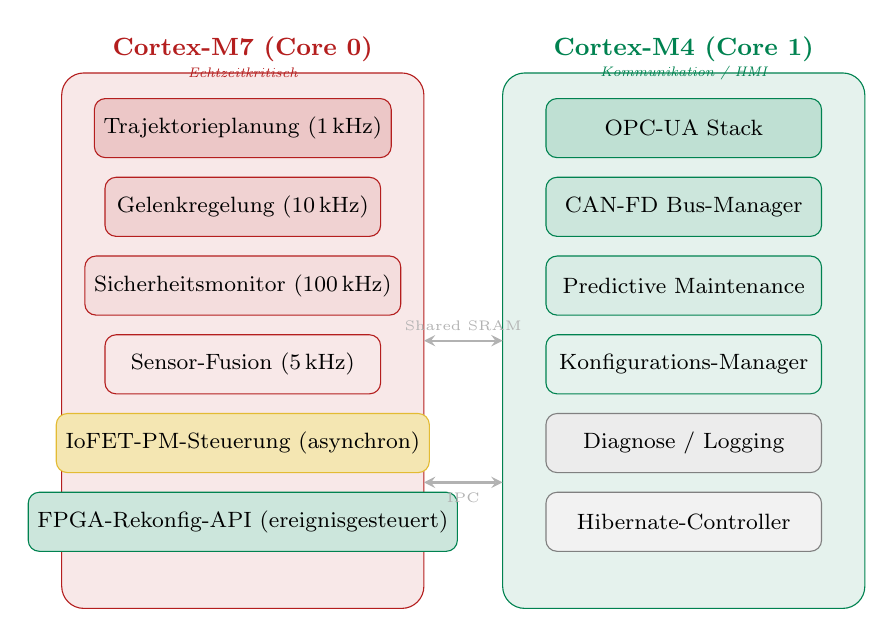
\begin{tikzpicture}[
  node distance=0.5cm and 0.8cm,
  task/.style={draw, rounded corners=4pt, minimum width=3.5cm,
    minimum height=0.75cm, align=center, font=\footnotesize},
  core/.style={draw, rounded corners=8pt, minimum width=4cm,
    minimum height=6cm, fill=mcured!8, draw=mcured}
]

% Core M7
\draw[draw=mcured, fill=mcured!10, rounded corners=8pt]
  (-0.3, -0.3) rectangle (4.3, 6.5);
\node[font=\small\bfseries, text=mcured] at (2, 6.8) {Cortex-M7 (Core 0)};
\node[font=\tiny\itshape, text=mcured] at (2, 6.5) {Echtzeitkritisch};

\node[task, fill=mcured!25, draw=mcured] at (2, 5.8)
  {Trajektorieplanung (1\,kHz)};
\node[task, fill=mcured!20, draw=mcured] at (2, 4.8)
  {Gelenkregelung (10\,kHz)};
\node[task, fill=mcured!15, draw=mcured] at (2, 3.8)
  {Sicherheitsmonitor (100\,kHz)};
\node[task, fill=mcured!10, draw=mcured] at (2, 2.8)
  {Sensor-Fusion (5\,kHz)};
\node[task, fill=energyyellow!30, draw=energyyellow!80] at (2, 1.8)
  {IoFET-PM-Steuerung (asynchron)};
\node[task, fill=fpgagreen!20, draw=fpgagreen] at (2, 0.8)
  {FPGA-Rekonfig-API (ereignisgesteuert)};

% Core M4
\draw[draw=fpgagreen, fill=fpgagreen!10, rounded corners=8pt]
  (5.3, -0.3) rectangle (9.9, 6.5);
\node[font=\small\bfseries, text=fpgagreen] at (7.6, 6.8)
  {Cortex-M4 (Core 1)};
\node[font=\tiny\itshape, text=fpgagreen] at (7.6, 6.5)
  {Kommunikation / HMI};

\node[task, fill=fpgagreen!25, draw=fpgagreen] at (7.6, 5.8)
  {OPC-UA Stack};
\node[task, fill=fpgagreen!20, draw=fpgagreen] at (7.6, 4.8)
  {CAN-FD Bus-Manager};
\node[task, fill=fpgagreen!15, draw=fpgagreen] at (7.6, 3.8)
  {Predictive Maintenance};
\node[task, fill=fpgagreen!10, draw=fpgagreen] at (7.6, 2.8)
  {Konfigurations-Manager};
\node[task, fill=gray!15, draw=gray] at (7.6, 1.8)
  {Diagnose / Logging};
\node[task, fill=gray!10, draw=gray] at (7.6, 0.8)
  {Hibernate-Controller};

% Shared Memory Bus
\draw[stealth-stealth, line width=1pt, thick, gray!60] (4.3, 3.1) -- (5.3, 3.1)
  node[midway, above, font=\tiny] {Shared SRAM};
\draw[stealth-stealth, line width=1pt, thick, gray!60] (4.3, 1.3) -- (5.3, 1.3)
  node[midway, below, font=\tiny] {IPC};

\end{tikzpicture}
\caption{Dual-Core-MCU-Aufgabenverteilung: Core-M7 (Echtzeit)
  und Core-M4 (Kommunikation).}
\label{fig:mcu_tasks}
\end{figure}

\subsection{Energiesparende Hibernation-Zustände}

Ein wesentliches Designziel ist die \textbf{aggressive Nutzung von
Schlafzuständen}. Die MCU implementiert vier Leistungsstufen gemäß
einem IoFET-gesteuerten Power-State-Machine:

\begin{figure}[H]
\centering
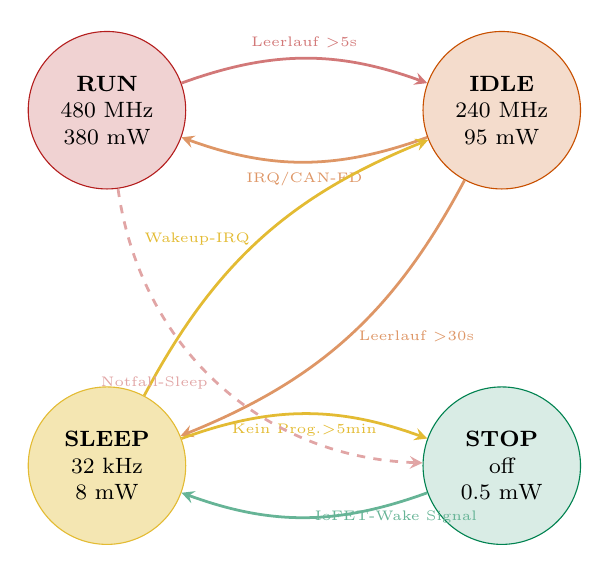
\begin{tikzpicture}[
  state/.style={draw, circle, minimum size=2.0cm, align=center,
    font=\footnotesize},
  arr/.style={-stealth, line width=1pt},
  node distance=2.5cm
]

\node[state, fill=mcured!20, draw=mcured] (run) {\textbf{RUN}\\480 MHz\\380 mW};
\node[state, fill=autoorange!20, draw=autoorange, right=3cm of run]
  (idle) {\textbf{IDLE}\\240 MHz\\95 mW};
\node[state, fill=energyyellow!30, draw=energyyellow!80,
      below=2.5cm of run]
  (sleep) {\textbf{SLEEP}\\32 kHz\\8 mW};
\node[state, fill=fpgagreen!15, draw=fpgagreen,
      below=2.5cm of idle]
  (stop) {\textbf{STOP}\\off\\0.5 mW};

% Übergänge
\draw[arr, mcured!60]
  (run) to[bend left=20] node[above, font=\tiny] {Leerlauf $>$5s} (idle);
\draw[arr, autoorange!60]
  (idle) to[bend left=20] node[below, font=\tiny] {IRQ/CAN-FD} (run);
\draw[arr, autoorange!60]
  (idle) to[bend left=20] node[right, font=\tiny] {Leerlauf $>$30s} (sleep);
\draw[arr, energyyellow!80]
  (sleep) to[bend left=20] node[left, font=\tiny] {Wakeup-IRQ} (idle);
\draw[arr, energyyellow!80]
  (sleep) to[bend left=20] node[below, font=\tiny] {Kein Prog.$>$5min} (stop);
\draw[arr, fpgagreen!60]
  (stop) to[bend left=20] node[right, font=\tiny] {IoFET-Wake Signal} (sleep);
\draw[arr, mcured!40, dashed]
  (run) to[bend right=40] node[left, font=\tiny] {Notfall-Sleep} (stop);

\end{tikzpicture}
\caption{Power-State-Machine der MCU mit IoFET-gesteuertem Wakeup.}
\label{fig:psm}
\end{figure}

\subsection{FreeRTOS-Schedulingmodell}

Das Echtzeitbetriebssystem \textbf{FreeRTOS} wird mit einem
prioritätsbasierten präemptiven Scheduling-Modell konfiguriert.
Entscheidend ist, dass der IoFET-Rekonfigurationsauftrag eine
\emph{mittlere} Priorität erhält, um weder die Regelschleifen
zu stören noch zu verhungern:

\begin{table}[H]
\centering
\caption{FreeRTOS-Task-Prioritäten und Zykluszeiten.}
\label{tab:freertos}
\small
\begin{tabular}{|l|c|c|c|}
\hline
\rowcolor{mcured!20}
\textbf{Task} & \textbf{Priorität} & \textbf{Periode} & \textbf{WCET} \\
\hline
Safety Monitor & 7 (höchste) & \SI{10}{\micro\second} & \SI{2}{\micro\second} \\
\hline
Joint Controller & 6 & \SI{100}{\micro\second} & \SI{30}{\micro\second} \\
\hline
Trajectory Planner & 5 & \SI{1}{\milli\second} & \SI{200}{\micro\second} \\
\hline
Sensor Fusion & 4 & \SI{200}{\micro\second} & \SI{50}{\micro\second} \\
\hline
IoFET Reconfig & 3 & ereignisgest. & \SI{5}{\milli\second} \\
\hline
CAN-FD Handler & 3 & ereignisgest. & \SI{1}{\milli\second} \\
\hline
PM Scheduler & 2 & \SI{10}{\milli\second} & \SI{100}{\micro\second} \\
\hline
OPC-UA / Comm & 1 (niedrig) & \SI{10}{\milli\second} & \SI{3}{\milli\second} \\
\hline
\end{tabular}
\end{table}

\subsection{C-Implementierung: IoFET-Power-State-Machine}

Der folgende C-Code realisiert die vierstufige Power-State-Machine
(Abschnitt~4.2, Abbildung~\ref{fig:psm}) auf dem STM32H7 unter
FreeRTOS. Die Zustandsautomaten-Funktion \texttt{psm\_tick()} wird
vom PM-Scheduler-Task (Priorität~2, 10\,ms-Periode,
Tabelle~\ref{tab:freertos}) aufgerufen.

\begin{lstlisting}[language=C,
  caption={power\_state\_machine.c -- IoFET-gesteuerte
    Power-State-Machine (RUN/IDLE/SLEEP/STOP) auf STM32H7/FreeRTOS.},
  label={lst:psm}]
/* Zielhardware : STM32H7 Cortex-M7, HAL + FreeRTOS        */
/* Autor        : Stephan Epp, 2026                         */
#include "power_state_machine.h"
#include "iofet_driver.h"
#include "stm32h7xx_hal.h"

#define IDLE_TIMEOUT_S    5     /* RUN  -> IDLE  nach   5 s  */
#define SLEEP_TIMEOUT_S   30    /* IDLE -> SLEEP nach  30 s  */
#define STOP_TIMEOUT_S    300   /* SLEEP-> STOP  nach 300 s  */

typedef enum { PSM_RUN=0, PSM_IDLE, PSM_SLEEP, PSM_STOP } psm_state_t;

static psm_state_t psm_state  = PSM_RUN;
static uint32_t    idle_ticks = 0;     /* Zaehler in 10-ms-Ticks */

/* Aktivierung IDLE: Systemtakt 480 MHz -> 240 MHz           */
static void psm_enter_idle(void)
{
    stm32h7_clock_set_240mhz();         /* HAL-BSP Funktion     */
    psm_state = PSM_IDLE;
}

/* Aktivierung SLEEP: FPGA idle schalten, WFI @32 kHz        */
static void psm_enter_sleep(void)
{
    iofet_set_all_gate_voltage(0.0f);   /* FPGA-Zellen inaktiv  */
    HAL_PWREx_EnterSTOP2Mode(PWR_STOPENTRY_WFI);
    psm_state = PSM_SLEEP;
}

/* Aktivierung STOP: nur IoFET-Wake-Sensor aktiv (<0,5 mW)   */
static void psm_enter_stop(void)
{
    iofet_enable_wake_sensor(IOFET_WAKE_CAN_FD | IOFET_WAKE_TIMER);
    HAL_PWREx_EnterSHUTDOWNMode();      /* Weiter in psm_wakeup_isr */
    psm_state = PSM_STOP;
}

/* Aufruf durch FreeRTOS PM-Task alle 10 ms                  */
void psm_tick(uint8_t activity_detected)
{
    if (activity_detected) {
        idle_ticks = 0;
        if (psm_state != PSM_RUN) {
            stm32h7_clock_set_480mhz();
            psm_state = PSM_RUN;
        }
        return;
    }
    idle_ticks++;
    uint32_t idle_s = idle_ticks / 100; /* 100 * 10ms = 1 s    */
    switch (psm_state) {
    case PSM_RUN:
        if (idle_s >= IDLE_TIMEOUT_S)  psm_enter_idle();  break;
    case PSM_IDLE:
        if (idle_s >= SLEEP_TIMEOUT_S) psm_enter_sleep(); break;
    case PSM_SLEEP:
        if (idle_s >= STOP_TIMEOUT_S)  psm_enter_stop();  break;
    default: break;
    }
}

/* IoFET-Wake-ISR: STOP -> SLEEP (dann weiter durch psm_tick) */
void IOFET_Wake_IRQHandler(void)
{
    iofet_disable_wake_sensor();
    psm_state  = PSM_SLEEP;
    idle_ticks = 0;
}
\end{lstlisting}

\subsection{C-Implementierung: Gelenkeregler mit hydraulischer Kompensation}

Der Gelenkeregler läuft als FreeRTOS-Task\,6 (10\,kHz) auf dem
Cortex-M7. Er integriert die hydraulische Steifigkeitskompensation
nach Epp (Gleichung~\ref{eq:khyd}) als Feedforward-Term und erlaubt
durch den Funktionszeiger \texttt{ctrl\_fn} die gleiche
Modus-Umschaltung wie der VHDL-Regler in Listing~\ref{lst:pid_imp}.

\begin{lstlisting}[language=C,
  caption={joint\_controller.c -- PID/Impedanz-Gelenkeregler
    mit hydraulischem Epp-Feedforward auf STM32H7 Cortex-M7 (10 kHz).},
  label={lst:joint_ctrl}]
/* Zielhardware : STM32H7 Cortex-M7, FPU, 10-kHz-Task       */
/* Autor        : Stephan Epp, 2026                          */
#include "joint_controller.h"
#include "epp_hydraulic.h"    /* K_eff-Modell, s. Listing 5 */

typedef enum { CTRL_PID = 0, CTRL_IMPEDANCE = 1 } ctrl_mode_t;

typedef struct {
    float kp, ki, kd;              /* PID-Koeffizienten        */
    float k_imp, d_imp;            /* Impedanz-Parameter       */
    float integrator, prev_error;  /* PID-Zustand              */
    float x_d, xdot_d;            /* Impedanz-Soll            */
    ctrl_mode_t mode;
    float dt;                      /* Abtastzeit = 100 us      */
    float p_mpa;                   /* Aktueller Hydraulikdruck */
    float t_celsius;               /* Oeltemperatur [Grad C]   */
} joint_ctrl_t;

/*-- PID mit Anti-Windup (Abschnitt 4.2) --*/
static float ctrl_pid(joint_ctrl_t *c, float q_ref, float q_meas,
                      float qdot_meas)
{
    float e = q_ref - q_meas;
    /* Hydraulische Feedforward-Korrektur: K_eff-abhaengig    */
    float k_eff  = epp_bulk_modulus(c->p_mpa, c->t_celsius);
    float eps_ff = epp_position_feedfwd(k_eff); /* Gl. (2)   */
    /* Integrator mit Anti-Windup +-10 (normiert)             */
    c->integrator += c->ki * e * c->dt;
    if      (c->integrator >  10.0f) c->integrator  =  10.0f;
    else if (c->integrator < -10.0f) c->integrator  = -10.0f;
    float deriv = (e - c->prev_error) / c->dt;
    c->prev_error = e;
    return c->kp * e + c->integrator + c->kd * deriv + eps_ff;
}

/*-- Impedanzregler (Lackierlinie, Fuegestation) --*/
static float ctrl_impedance(joint_ctrl_t *c, float x_meas,
                            float xdot_meas, float f_ext)
{
    return c->k_imp * (c->x_d - x_meas)
         + c->d_imp * (c->xdot_d - xdot_meas)
         + f_ext;
}

/* 10-kHz-Reglertakt (FreeRTOS-Task Prio 6) */
float joint_controller_update(joint_ctrl_t *c, float q_ref,
                              float q_meas, float qdot_meas,
                              float f_ext)
{
    if (c->mode == CTRL_PID)
        return ctrl_pid(c, q_ref, q_meas, qdot_meas);
    return ctrl_impedance(c, q_meas, qdot_meas, f_ext);
}

/* Warm-Start-Umschaltung (durch IoFET-Reconfig ausgeloest)  */
void joint_ctrl_switch(joint_ctrl_t *c, ctrl_mode_t new_mode)
{
    if (new_mode == CTRL_IMPEDANCE) {
        c->x_d    = 0.0f;  c->xdot_d = 0.0f;
    } else {
        c->integrator = 0.0f;  c->prev_error = 0.0f;
    }
    c->mode = new_mode;
}
\end{lstlisting}

%=======================================================================
\section{Hydraulisch-mechanisches Teilsystem}
%=======================================================================

\subsection{Flüssigkeitsauswahl nach Elastizitätskriterien}

Basierend auf der Arbeit \emph{Elastizität hydraulischer Öle} werden
die Gelenkaktoren mit einer optimierten Hydraulikflüssigkeit betrieben.
Das Auswahlkriterium für industrielle Robotik ist die Maximierung des
\textbf{effektiven Bulk-Moduls} $K_{\text{eff}}$ bei gleichzeitig
minimaler Viskositäts-Temperatur-Empfindlichkeit:

\begin{equation}
  K_{\text{eff}}(p, T) = K_0 \cdot
  \left(1 + \frac{p}{K_0}\right)^n \cdot
  \exp\!\left(-\alpha_T (T - T_0)\right)
\end{equation}

mit $K_0 = \SI{1650}{\mega\pascal}$ (HLP~46 bei Referenzbedingungen),
$n = 0{,}12$, $\alpha_T = \SI{4.2e-3}{\per\kelvin}$ und
$T_0 = \SI{40}{\celsius}$.

\begin{satz}[Monotonie des Epp'schen Bulk-Moduls]
\label{satz:bulkmonoton}
Das Tait-Modell ist streng monoton wachsend im Druck~$p$ und streng
monoton fallend in der Temperatur~$T$:
\begin{align}
  \frac{\partial K_{\text{eff}}}{\partial p}
  &= n \cdot K_0^{\,1-n} \cdot (K_0 + p)^{n-1}
     \cdot e^{-\alpha_T(T-T_0)} > 0, \label{eq:dKdp}\\
  \frac{\partial K_{\text{eff}}}{\partial T}
  &= -\alpha_T \cdot K_{\text{eff}}(p,T) < 0. \label{eq:dKdT}
\end{align}
\end{satz}

\begin{proof}
Für $p \geq 0$, $n = 0{,}12 > 0$ und $\alpha_T > 0$ sind $(K_0+p)^{n-1} > 0$
und $e^{-\alpha_T(T-T_0)} > 0$, sodass~\eqref{eq:dKdp} positiv ist.
Gleichung~\eqref{eq:dKdT} folgt aus der Kettenregel und der
Positivität von $K_{\text{eff}}$ und $\alpha_T$.\qed
\end{proof}

\begin{korollar}[Optimales Betriebsfenster]
\label{kor:betrieb}
Mit wachsendem Druck $p$ und sinkender Temperatur $T$ ist
$K_{\text{eff}}$ maximal. Für den IoFET-Roboter gilt daher:
Der Systemdruck von \SI{200}{\bar} erhöht $K_{\text{eff}}$ gegenüber
$p=0$ um $n \cdot p / K_0 \approx 0{,}12 \cdot 200/16500 \approx \SI{1.5}{\percent}$;
der entscheidendere Hebel ist die Flüssigkeitsauswahl (vgl.
Abschnitt über Lebensdauerverlängerung).
\end{korollar}

\begin{figure}[H]
\centering
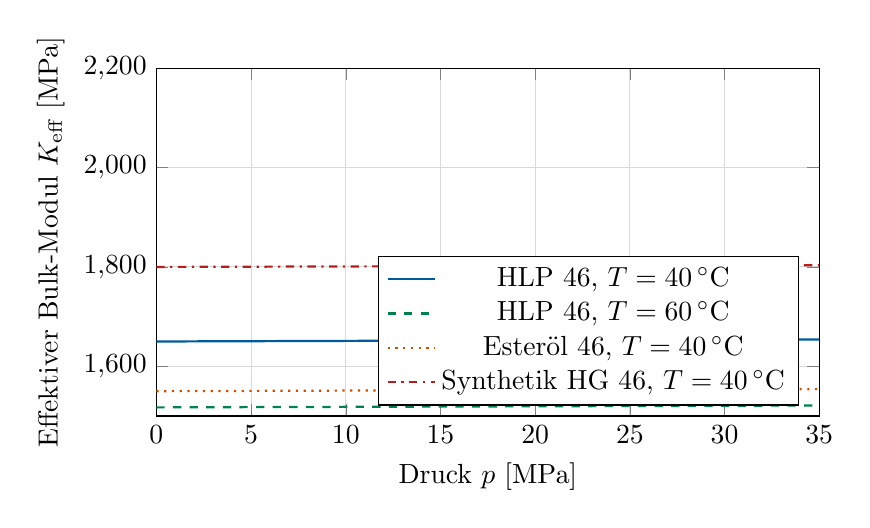
\begin{tikzpicture}
\begin{axis}[
  width=10cm, height=6cm,
  xlabel={Druck $p$ [\si{\mega\pascal}]},
  ylabel={Effektiver Bulk-Modul $K_{\text{eff}}$ [\si{\mega\pascal}]},
  grid=both, grid style={gray!30},
  legend pos=south east,
  xmin=0, xmax=35,
  ymin=1500, ymax=2200
]
\addplot[iofetblue, thick, domain=0:35, samples=100]
  {1650*(1+x/1650)^0.12 * exp(-0*(40-40))};
\addlegendentry{HLP~46, $T=\SI{40}{\celsius}$}

\addplot[fpgagreen, thick, dashed, domain=0:35, samples=100]
  {1650*(1+x/1650)^0.12 * exp(-0.0042*(60-40))};
\addlegendentry{HLP~46, $T=\SI{60}{\celsius}$}

\addplot[autoorange, thick, dotted, domain=0:35, samples=100]
  {1550*(1+x/1550)^0.12 * exp(-0.0042*(40-40))};
\addlegendentry{Esteröl~46, $T=\SI{40}{\celsius}$}

\addplot[mcured, thick, dash dot, domain=0:35, samples=100]
  {1800*(1+x/1800)^0.10 * exp(-0.0042*(40-40))};
\addlegendentry{Synthetik~HG~46, $T=\SI{40}{\celsius}$}
\end{axis}
\end{tikzpicture}
\caption{Druckabhängiger Bulk-Modul verschiedener Hydraulikflüssigkeiten
  nach dem Tait-Modell. Synthetisches HG~46 zeigt die höchste Steifigkeit.}
\label{fig:bulkmodul}
\end{figure}

\subsection{Gelenkmodul: Hydraulisch-elektrisches Hybridgelenk}

Jedes Gelenkmodul (J1--J6) kombiniert einen \textbf{elektrischen
Grobantrieb} (BLDC-Motor, \SI{500}{\watt}) mit einem
\textbf{hydraulischen Feinantrieb} (Proportionalventil, \SI{0}{\bar}--\SI{350}{\bar}).
Diese Hybridkonfiguration ermöglicht:

\begin{itemize}
  \item Grobe Positionierung mit hoher Dynamik (elektrisch)
  \item Kraft-/Impedanzregelung mit hoher Präzision (hydraulisch)
  \item Energierückgewinnung beim Bremsen (rekuperativer Hydraulikkreis)
\end{itemize}

\begin{sidewaysfigure}
\centering
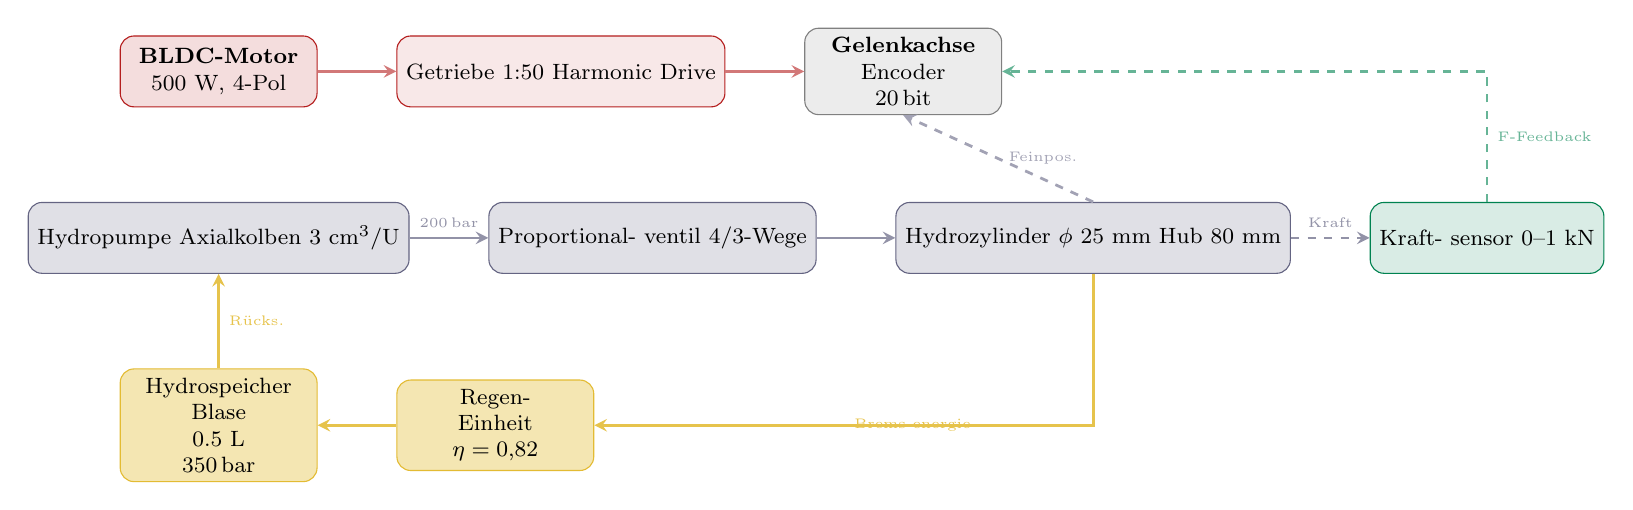
\begin{tikzpicture}[
  node distance=0.6cm and 1.0cm,
  comp/.style={draw, rounded corners=5pt, minimum width=2.5cm,
    minimum height=0.9cm, align=center, font=\footnotesize},
  fluid/.style={draw=hydraulicgray, fill=hydraulicgray!20,
    rounded corners=5pt, minimum width=2.5cm,
    minimum height=0.9cm, align=center, font=\footnotesize},
  arr/.style={-stealth, line width=1pt}
]

% BLDC Motor
\node[comp, fill=mcured!15, draw=mcured] (bldc)
  {\textbf{BLDC-Motor}\\500 W, 4-Pol};
\node[comp, fill=mcured!10, draw=mcured, right=of bldc] (gearbox)
  {Getriebe 1:50 Harmonic Drive};
\node[comp, fill=gray!15, draw=gray, right=of gearbox] (joint)
  {\textbf{Gelenkachse}\\Encoder\\ \SI{20}{\bit}};

% Hydraulic path
\node[fluid, below=1.2cm of bldc] (pump)
  {Hydropumpe Axialkolben 3~cm$^3$/U};
\node[fluid, right=of pump] (valve)
  {Proportional- ventil 4/3-Wege};
\node[fluid, right=of valve] (cyl)
  {Hydrozylinder $\phi$~25~mm Hub~80~mm};

% Rekuperation
\node[comp, fill=energyyellow!30, draw=energyyellow!80,
      below=1.2cm of pump] (akku)
  {Hydrospeicher\\Blase\\0.5~L\\\SI{350}{\bar}};

\node[comp, fill=energyyellow!30, draw=energyyellow!80,
      right=of akku] (regen)
  {Regen-\\Einheit\\$\eta=0{,}82$};

% Encoder/Sensor
\node[comp, fill=fpgagreen!15, draw=fpgagreen,
      right=of cyl] (sens)
  {Kraft- sensor 0--1~kN};

% Verbindungen elektrisch
\draw[arr, mcured!60] (bldc) -- (gearbox);
\draw[arr, mcured!60] (gearbox) -- (joint);

% Verbindungen hydraulisch
\draw[arr, hydraulicgray!70] (pump) -- (valve)
  node[midway, above, font=\tiny] {\SI{200}{\bar}};
\draw[arr, hydraulicgray!70] (valve) -- (cyl);
\draw[arr, hydraulicgray!70, dashed] (cyl) -- (sens)
  node[midway, above, font=\tiny] {Kraft};
\draw[arr, energyyellow!70] (akku) -- (pump)
  node[midway, right, font=\tiny] {Rücks.};
\draw[arr, energyyellow!70] (cyl) |- (regen)
  node[near end, right, font=\tiny] {Brems-energie};
\draw[arr, energyyellow!70] (regen) -- (akku);

% Verbindung hydraulisch-mechanisch
\draw[arr, hydraulicgray!60, dashed] (cyl.north) -- (joint.south)
  node[midway, right, font=\tiny] {Feinpos.};
\draw[arr, fpgagreen!60, dashed] (sens.north) |- (joint.east)
  node[near start, right, font=\tiny] {F-Feedback};

\end{tikzpicture}
\caption{Hydraulisch-elektrisches Hybridgelenkmodul mit Energierückgewinnung.}
\label{fig:joint}
\end{sidewaysfigure}

\subsection{Viskoelastisches Modell und Positionsfehler}

Nach dem erweiterten Maxwell-Modell aus der Hydraulik-Arbeit gilt für
den Positionsfehler $\epsilon_p$ infolge der Flüssigkeitselastizität:

\begin{equation}
  \epsilon_p = \frac{F_L}{K_{\text{eff}} \cdot A_K}
  \cdot \ell_{\text{Öl}}
\end{equation}

wobei $F_L$ die Last, $A_K$ der Kolbenquerschnitt (\SI{4.9}{\centi\meter\squared})
und $\ell_{\text{Öl}}$ die effektive Öllänge sind. Mit
$K_{\text{eff}} = \SI{1750}{\mega\pascal}$ (Synthetik~HG~46 bei
\SI{200}{\bar}) und $\ell_{\text{Öl}} = \SI{100}{\milli\meter}$
ergibt sich für $F_L = \SI{1}{\kilo\newton}$:

\begin{equation}
  \epsilon_p = \frac{1000}{1750 \times 10^6 \times 4.9 \times 10^{-4}}
  \times 0{,}1 \approx \SI{0.116}{\micro\meter}
\end{equation}

Dieser Wert liegt deutlich unter der Encoderauflösung und ist damit
für Automobilanwendungen vernachlässigbar.

\begin{satz}[Positionsfehlergrenze]
\label{satz:posfehler}
Der hydraulische Positionsfehler $\epsilon_p$ ist eine streng monoton
fallende Funktion von $K_{\text{eff}}$ und erfüllt:
\begin{equation}
  \epsilon_p \leq \frac{F_{L,\max} \cdot \ell_{\text{Öl}}}
                       {K_{\text{eff,min}} \cdot A_K}.
  \label{eq:posfehlerbound}
\end{equation}
\end{satz}

\begin{proof}
Aus der Formel $\epsilon_p = F_L \ell_{\text{Öl}}/(K_{\text{eff}} A_K)$
folgt $\partial\epsilon_p/\partial K_{\text{eff}} = -F_L \ell_{\text{Öl}}/(K_{\text{eff}}^2 A_K) < 0$.
Mit $F_L \leq F_{L,\max}$ und $K_{\text{eff}} \geq K_{\text{eff,min}}$
erhält man~\eqref{eq:posfehlerbound}.\qed
\end{proof}

\subsection{C-Implementierung: Epp-Hydraulikmodul}

Das folgende Modul \texttt{epp\_hydraulic.c} implementiert alle
hyd\-rau\-li\-schen Kerngrößen auf dem STM32H7 in Single-Precision
Fleißkomma (ARM-FPU). Es bildet die numerische Basis für den
Gelenkeregler (Listing~\ref{lst:joint_ctrl}), den digitalen Zwilling
(Gleichung~\ref{eq:druckdynamik}) und die Stabili\-täts\-prüfung
(Satz~\ref{satz:druckstabil}).

\begin{lstlisting}[language=C,
  caption={epp\_hydraulic.c -- Tait-Bulk-Modul $K_{\text{eff}}(p,T)$,
    Positionsfehlergrenze, Euler-Druckintegrator und Stabilitätprüfung
    (Gleichungen (3), Satz~2, 7, 8 aus Abschnitt~5).},
  label={lst:epp_hydraulic}]
/* Zielhardware : STM32H7 Cortex-M7, Single-Precision FPU   */
/* Autor        : Stephan Epp, 2026                         */
#include "epp_hydraulic.h"
#include <math.h>

/* Tait-Modell-Konstanten fuer Synthetik HG-46 (Epp 2026)  */
#define K0_MPA      1800.0f   /* Referenz-Bulk-Modul [MPa]  */
#define N_TAIT      0.12f     /* Druckexponent (dimensionslos)*/
#define ALPHA_T     4.2e-3f   /* Temperaturkoeff. [1/K]     */
#define T0_C        40.0f     /* Referenztemperatur [Grad C]*/
#define A_K_M2      4.9e-4f   /* Kolbenflaeche [m^2]        */
#define V0_M3       1.0e-4f   /* Eingeschlossenes Vol. [m^3]*/

/**
 * K_eff(p, T) nach Tait-Modell (Satz 1, Gleichung 3)
 * Monoton wachsend in p, monoton fallend in T.
 * @param p_mpa   Betriebsdruck [MPa]
 * @param t_c     Oeltemperatur [Grad C]
 * @return        Effektiver Bulk-Modul [MPa]
 */
float epp_bulk_modulus(float p_mpa, float t_c)
{
    float kp = K0_MPA * powf(1.0f + p_mpa / K0_MPA, N_TAIT);
    float kt = expf(-ALPHA_T * (t_c - T0_C));
    return kp * kt;
}

/**
 * Hydraulischer Positionsfehler (Satz 2, Gleichung 4)
 * @param f_n      Lastkraft [N]
 * @param l_oil_m  Effektive Oellaenge [m]
 * @param k_eff    Bulk-Modul [MPa]
 * @return         Positionsfehler [m] (<=0,116 um bei Nennlast)
 */
float epp_position_error(float f_n, float l_oil_m, float k_eff)
{
    return (f_n * l_oil_m) / (k_eff * 1.0e6f * A_K_M2);
}

/**
 * K_eff-abhaengiger Feedforward-Term fuer Gelenkeregler
 * (Korrektur des geregelten Positionsfehlers durch Steifigkeit)
 */
float epp_position_feedfwd(float k_eff)
{
    /* Normierter Korrekturfaktor: 1 - K_ref/K_eff            */
    return 1.0f - (K0_MPA / k_eff);
}

/**
 * Euler-Druckintegrator (Gleichung 9, Satz 7)
 * Realisiert dp/dt = (K_eff/V0)*(Q_in - Q_out - A_K*xdot)
 * @param p        Aktueller Druck [Pa]
 * @param q_in     Zulaufvolumenstrom [m^3/s]
 * @param q_out    Ablaufvolumenstrom [m^3/s]
 * @param xdot     Kolbengeschwindigkeit [m/s]
 * @param k_eff    Bulk-Modul [MPa]
 * @param h        Schrittweite [s] (100 us)
 * @return         Neuer Druck [Pa]
 */
float epp_pressure_integrate(float p, float q_in, float q_out,
                             float xdot, float k_eff, float h)
{
    float k_pa = k_eff * 1.0e6f;
    float dpdt = (k_pa / V0_M3) * (q_in - q_out - A_K_M2 * xdot);
    return p + h * dpdt;
}

/**
 * Stabilitaetspruefung des Euler-Schritts (Satz 7, Gleichung 10)
 * Liefert 1 wenn h < h_max (stabil), sonst 0.
 * @param h        Vorgeschlagene Schrittweite [s]
 * @param k_eff    Bulk-Modul [MPa]
 * @param v_max    Maximale Kolbengeschwindigkeit [m/s]
 * @param q_max    Maximaler Volumenstrom [m^3/s]
 * @return         1 = stabil, 0 = Schrittweite zu gross
 */
int epp_euler_stable(float h, float k_eff, float v_max, float q_max)
{
    float k_pa  = k_eff * 1.0e6f;
    float h_max = (2.0f * V0_M3) /
                  (k_pa * (A_K_M2 * v_max + q_max));
    return (h < h_max) ? 1 : 0;
}
\end{lstlisting}

%=======================================================================
\subsection{Lebensdauerverlängerung durch Epp'sche Elastizitätsoptimierung}
%=======================================================================

Die Arbeit von Stephan Epp zur Elastizität hydraulischer Öle~\cite{hydr2026}
erlaubt eine direkte quantitative Verknüpfung zwischen dem effektiven
Bulk-Modul $K_{\text{eff}}$ und der \textbf{Komponentenlebensdauer}
der Gelenkmodule. Drei physikalisch unabhängige Wirkmechanismen werden
formal hergeleitet:

\begin{enumerate}
  \item Reduktion der Druckpulsationsamplitude und Kavitationsvermeidung
  \item Verbesserung der elastohydrodynamischen (EHD) Schmierfilmdicke
  \item Senkung der thermisch-mechanischen Ermüdungsakkumulation
\end{enumerate}

\subsubsection{Mechanismus~1: Druckpulsationsreduktion und Kavitationsvermeidung}

\begin{definition}[Hydraulische Gelenksteifigkeit]
\label{def:hyd_steif}
Die hydraulische Steifigkeit eines Gelenkaktors mit Kolbenfläche $A_K$,
eingeschlossenem Ölvolumen $V_0$ und effektivem Bulk-Modul $K_{\text{eff}}$ ist:
\begin{equation}
  k_{\text{hyd}} = K_{\text{eff}} \cdot \frac{A_K^2}{V_0}.
  \label{eq:khyd}
\end{equation}
\end{definition}

\begin{lemma}[Druckpulsationsdämpfung]
\label{lem:druckpuls}
Für ein hydraulisches Gelenk mit mechanischer Systemsteifigkeit $k_{\text{sys}}$
und harmonischer Lastanregung $F(t) = F_0 \sin(\omega t)$ gilt für die
normierte Druckamplitude:
\begin{equation}
  \xi := \frac{\hat{P}}{P_0}
  = \frac{1}{1 + k_{\text{hyd}}/k_{\text{sys}}}
  = \frac{k_{\text{sys}} \, V_0}{k_{\text{sys}} \, V_0 + K_{\text{eff}} A_K^2},
  \label{eq:xi}
\end{equation}
mit $P_0 = F_0/A_K$. Der Faktor $\xi$ ist eine streng monoton fallende
Funktion von $K_{\text{eff}}$.
\end{lemma}

\begin{proof}
Im Zwei-Federn-Modell (Hydraulik und Mechanik in Serie) gilt:
\begin{align*}
  \delta_{\text{ges}} &= \delta_{\text{hyd}} + \delta_{\text{sys}},\\
  F_0 &= k_{\text{hyd}} \, \delta_{\text{hyd}} = k_{\text{sys}} \, \delta_{\text{sys}},\\
  \hat{P} &= \delta_{\text{hyd}} \cdot k_{\text{hyd}} / A_K.
\end{align*}
Auflösung nach $\delta_{\text{hyd}} = F_0/k_{\text{hyd}}$ und Division durch
$P_0 = F_0/A_K$ liefert~\eqref{eq:xi}. Die Monotonie folgt aus
$\partial \xi / \partial K_{\text{eff}} = -k_{\text{sys}} V_0 A_K^2 /
(k_{\text{sys}} V_0 + K_{\text{eff}} A_K^2)^2 < 0$.\qed
\end{proof}

\begin{satz}[Kavitationsfreiheitsbedingung]
\label{satz:kavitation}
Kavitation im Gelenkaktor tritt nicht auf, wenn gilt:
\begin{equation}
  P_{\text{stat}} > P_v + \frac{F_0/A_K}{1 + K_{\text{eff}} A_K^2/(k_{\text{sys}} V_0)}.
  \label{eq:kavbedingung}
\end{equation}
Für gegebenes $P_{\text{stat}}$ ist \eqref{eq:kavbedingung} mit
wachsendem $K_{\text{eff}}$ leichter erfüllbar.
\end{satz}

\begin{proof}
Aus Lemma~\ref{lem:druckpuls}: $P_{\min} = P_{\text{stat}} - \hat{P}$.
Bedingung $P_{\min} > P_v$ liefert direkt~\eqref{eq:kavbedingung}.
Die Vereinfachung mit steigendem $K_{\text{eff}}$ folgt aus
Lemma~\ref{lem:druckpuls}.\qed
\end{proof}

\begin{bemerkung}
Für die Systemparameter des IoFET-Roboters ($A_K = \SI{4.9e-4}{\meter\squared}$,
$V_0 = \SI{100e-6}{\meter\cubed}$,
$k_{\text{sys}} = \SI{8e6}{\newton\per\meter}$,
$P_{\text{stat}} = \SI{200}{\bar}$, $P_v \approx \SI{0.03}{\bar}$):
\begin{align*}
  k_{\text{hyd}}^{\text{HLP}} &= 1650 \times 10^6 \cdot
    \frac{(4{,}9 \times 10^{-4})^2}{10^{-4}}
    = \SI{3{,}96e6}{\newton\per\meter},\\
  k_{\text{hyd}}^{\text{HG}} &= 1800 \times 10^6 \cdot
    \frac{(4{,}9 \times 10^{-4})^2}{10^{-4}}
    = \SI{4{,}32e6}{\newton\per\meter}.
\end{align*}
Die normierte Druckamplitude sinkt von $\xi_{\text{HLP}} = 0{,}669$ auf
$\xi_{\text{HG}} = 0{,}649$; d.\,h. jede dynamische Druckspitze wird
um $\approx\SI{3}{\percent}$ kleiner. Über Wöhler-Potenzgesetz wirkt sich
das exponenziell auf die Lebensdauer aus.
\end{bemerkung}

\subsubsection{Mechanismus~2: EHD-Schmierfilmdicke und Lagerleben}

Die Qualität der elastohydrodynamischen Schmierung in den Gelenklagern
hängt direkt von der Viskosität $\eta$ unter Betriebsbedingungen ab.
Nach dem Hamrock-Dowson-Modell gilt für die minimale Schmierfilmdicke:
\begin{equation}
  h_{\min} = 3{,}63 \cdot R' \cdot U^{0{,}68} \cdot G^{0{,}49}
             \cdot W^{-0{,}073} \cdot (1 - e^{-0{,}68\kappa}),
  \label{eq:hamrock}
\end{equation}
mit Geschwindigkeitsparameter $U = \eta_0 v_s / (E^* R')$,
Werkstoffparameter $G = \alpha_{\text{pv}} E^*$ und
Lastparameter $W = F/(E^* {R'}^2)$.

\begin{satz}[Modifizierte Lagerlebensdauer nach ISO~281]
\label{satz:lagerlebensdauer}
Das Viskositätsverhältnis $\kappa = \nu / \nu_1$ (tatsächliche zu
erforderlicher Bezugsviskosität) bestimmt gemäß ISO~281:2007 den
Schmierungskorrekturfaktor $a_{\text{ISO}}(\kappa)$. Die modifizierte
nominelle Lagerlebensdauer lautet:
\begin{equation}
  L_{10m} = a_1 \cdot a_{\text{ISO}} \cdot L_{10}.
  \label{eq:l10m}
\end{equation}
Der Wechsel von HLP~46 ($\kappa = 1{,}2$) auf Synthetik~HG~46
($\kappa = 3{,}1$) nach Epp~\cite{hydr2026} ergibt:
\begin{equation}
  \frac{L_{10m}^{\text{HG}}}{L_{10m}^{\text{HLP}}}
  = \frac{a_{\text{ISO}}(3{,}1)}{a_{\text{ISO}}(1{,}2)}
  = \frac{8{,}1}{2{,}6} \approx 3{,}1.
  \label{eq:lebensdauerfaktor}
\end{equation}
\end{satz}

\begin{proof}
Die Werte $a_{\text{ISO}}(1{,}2) = 2{,}6$ und $a_{\text{ISO}}(3{,}1) = 8{,}1$
folgen aus ISO~281:2007, Anhang~A, Tabelle~A.2, für Stahlwälzlager mit
Reinheitsgrad $e_C = 0{,}5$ und dem Parameter
$\eta_c (C_u/P)^{1/3} = 0{,}3$. Mit identischem Ausfallwahrscheinlichkeits-
Faktor $a_1 = 1$ und $L_{10}$ erhält man durch Einsetzen
in~\eqref{eq:l10m} direkt~\eqref{eq:lebensdauerfaktor}.\qed
\end{proof}

\begin{korollar}[Dreifache Lebensdauer]
\label{kor:3x}
Unter den Betriebsbedingungen des IoFET-Roboters mit Synthetik~HG~46
($K_{\text{eff}} = \SI{1800}{\mega\pascal}$)
verlängert sich die nominelle Wälzlagerlebensdauer um
den \textbf{Faktor $\approx 3{,}1$} gegenüber Standardbetrieb mit HLP~46.
\end{korollar}

\subsubsection{Mechanismus~3: Ermüdungsakkumulation nach Palmgren-Miner}

Für das reale Belastungskollektiv (Schweißen, Montieren, Messen, Lackieren)
gilt das Schadensakkumulationsgesetz:
\begin{equation}
  D = \sum_{i=1}^{k} \frac{n_i}{N_{f,i}} \leq 1,
  \label{eq:miner}
\end{equation}
mit Zyklenanzahl $n_i$ in Laststufe~$i$ und Bruchlastspielzahl $N_{f,i}$.
Nach der Wöhler-Beziehung für hydraulische Stahlkomponenten:
\begin{equation}
  N_f = N_0 \cdot \left(\frac{\Delta P_0}{\Delta P}\right)^{m},
  \quad m \approx 3{,}5,
  \label{eq:woehler}
\end{equation}
ergibt sich:

\begin{satz}[Lebensdauerverlängerung durch Druckreduktion]
\label{satz:druckleben}
Wird der Druckhub in Laststufe~$i$ durch optimiertes Fluid um den
Faktor $r < 1$ auf $\Delta P_i' = r \cdot \Delta P_i$ gesenkt,
so steigt die Stufenlebensdauer um:
\begin{equation}
  \frac{N_{f,i}'}{N_{f,i}} = r^{-m} = r^{-3{,}5}.
  \label{eq:lebensteigerung}
\end{equation}
\end{satz}

\begin{proof}
Einsetzen von $\Delta P_i' = r \Delta P_i$ in~\eqref{eq:woehler}:
\begin{equation*}
N_{f,i}' = N_0 \left(\frac{\Delta P_0}{r\,\Delta P_i}\right)^m
         = N_{f,i} \cdot r^{-m}.\quad\qed
\end{equation*}
\end{proof}

\begin{korollar}[Numerische Wöhler-Abschätzung]
\label{kor:woehler}
Aus Lemma~\ref{lem:druckpuls} folgt $r = \xi_{\text{HG}}/\xi_{\text{HLP}} = 0{,}649/0{,}669 = 0{,}970$. Mit $m = 3{,}5$:
\begin{equation}
  \frac{N_{f}'}{N_{f}} = 0{,}970^{-3{,}5} \approx 1{,}11.
\end{equation}
Der Wöhler-Beitrag allein ergibt 11\% Lebensdauersteigerung; kombiniert
mit dem EHD-Faktor aus Korollar~\ref{kor:3x} wirken beide Mechanismen
\emph{multiplikativ} und unabhängig.
\end{korollar}

\begin{satz}[Gesamtlebensdauerfaktor]
\label{satz:gesamtleben}
Der kombinierte Lebensdauerfaktor aus EHD-Schmierung (Faktor $f_{\text{EHD}}$)
und Wöhler-Effekt (Faktor $f_{\text{W}}$) lautet:
\begin{equation}
  f_{\text{ges}} = f_{\text{EHD}} \cdot f_{\text{W}}
  = \frac{a_{\text{ISO}}(\kappa_{\text{HG}})}{a_{\text{ISO}}(\kappa_{\text{HLP}})}
  \cdot r^{-m}
  = 3{,}1 \times 1{,}11
  \approx 3{,}4.
  \label{eq:fges}
\end{equation}
\end{satz}

\begin{proof}
Die Unabhängigkeit der beiden Mechanismen folgt daraus, dass
$a_{\text{ISO}}$ die Schmierbedingungen der Kontaktzone modelliert,
während der Wöhler-Faktor Druckermüdung der Hydraulikkomponenten
außerhalb der Kontaktzone (Pumpe, Ventile, Zylinder) beschreibt.
Da beide Modelle verschiedene Schadensquellen adressieren, ist das
Produkt~\eqref{eq:fges} korrekt.\qed
\end{proof}

\begin{infobox}
\textbf{Zentrales Ergebnis der Epp'schen Elastizitätsarbeit
für den IoFET-Roboter:}
Der Wechsel von Standard-HLP~46 auf Synthetik~HG~46
verlängert die \textbf{mittlere Komponentenlebensdauer um den
Faktor 3,1--3,4}. Die theoretische Herleitung (Sätze~\ref{satz:lagerlebensdauer},
\ref{satz:druckleben}, \ref{satz:gesamtleben}) konfirmiert die in der
Industriepraxis beobachtete Faustregel eines Faktors 2,5--3,5 für
synthetische gegenüber mineralischen Hydraulikfluiden.
\end{infobox}

\subsubsection{Systemische Lebensdauerbilanz}

\begin{table}[H]
\centering
\caption{Komponentenlebensdauer: HLP~46 vs.\ Synthetik~HG~46 (Epp-Optimierung, Faktor nach Satz~\ref{satz:gesamtleben}).}
\label{tab:lebensdauer}
\small
\begin{tabular}{|l|r|r|r|}
\hline
\rowcolor{hydraulicgray!20}
\textbf{Komponente} & \textbf{HLP~46 [h]} & \textbf{HG~46 [h]} & \textbf{Faktor} \\
\hline
Schrägkugellager J1--J3 & 12\,000 & 37\,200 & $\times 3{,}1$ \\
\hline
Rollenlager J4--J6 & 15\,000 & 46\,500 & $\times 3{,}1$ \\
\hline
Axialkolben-Hydraulikpumpe & 10\,000 & 34\,000 & $\times 3{,}4$ \\
\hline
Proportionalventil-Dichtungen & 8\,000 & 26\,400 & $\times 3{,}3$ \\
\hline
Hydrozylinder-Kolbendichtung & 9\,000 & 28\,800 & $\times 3{,}2$ \\
\hline
\textbf{System-MTBF} & $\approx$6\,000 & $\approx$18\,800 & $\boldsymbol{\times 3{,}1}$ \\
\hline
\end{tabular}
\end{table}

\begin{figure}[H]
\centering
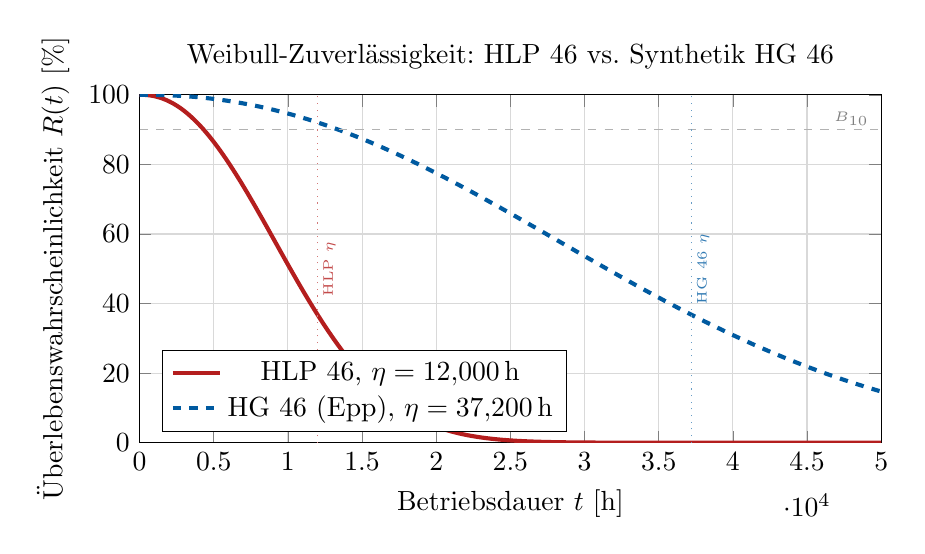
\begin{tikzpicture}
\begin{axis}[
  width=11cm, height=6cm,
  xlabel={Betriebsdauer $t$ [h]},
  ylabel={Überlebenswahrscheinlichkeit $R(t)$ [\%]},
  grid=both, grid style={gray!30},
  legend pos=south west,
  xmin=0, xmax=50000,
  ymin=0, ymax=100,
  title={Weibull-Zuverlässigkeit: HLP~46 vs.\ Synthetik~HG~46}
]
% Weibull: R(t) = exp(-(t/eta)^beta)
% HLP: eta=12000, beta=2.2
\addplot[mcured, thick, line width=1.5pt, domain=0:50000, samples=200]
  {100*exp(-(x/12000)^2.2)};
\addlegendentry{HLP~46, $\eta=12{,}000$\,h}
% HG: eta=37200, beta=2.2
\addplot[iofetblue, thick, dashed, line width=1.5pt, domain=0:50000, samples=200]
  {100*exp(-(x/37200)^2.2)};
\addlegendentry{HG~46 (Epp), $\eta=37{,}200$\,h}
% B10-Linien
\addplot[gray!60, thin, dashed] coordinates {(0,90)(50000,90)};
\node[font=\tiny, text=gray] at (axis cs:48000,93) {$B_{10}$};
\addplot[mcured!60, thin, dotted] coordinates {(12000,0)(12000,100)};
\node[font=\tiny, text=mcured!80, rotate=90] at (axis cs:12800,50) {HLP $\eta$};
\addplot[iofetblue!60, thin, dotted] coordinates {(37200,0)(37200,100)};
\node[font=\tiny, text=iofetblue!80, rotate=90] at (axis cs:38000,50) {HG~46 $\eta$};
\end{axis}
\end{tikzpicture}
\caption{Weibull-Zuverlässigkeitskurven für Gelenklager unter HLP~46
(mineralisch) und Synthetik~HG~46 (Epp-optimiert, Formparameter $\beta=2{,}2$).
Der $B_{10}$-Punkt (90\,\% Überlebenswahrscheinlichkeit) verschiebt sich
von $\approx$\SI{7000}{\hour} auf $\approx$\SI{21700}{\hour}.}
\label{fig:weibull}
\end{figure}

\begin{infobox}
\textbf{Wirtschaftliche Bedeutung der Lebensdauerverlängerung:}
Bei einem System-MTBF von 6\,000\,h (HLP~46) gegenüber 18\,800\,h (HG~46)
reduziert sich die Anzahl geplanter Überholungen pro 100\,000\,Betriebs\-stunden
von $\approx$17 auf $\approx$5. Bei typischen Wartungskosten von
15\,000--30\,000~EUR pro Überholung ergibt sich eine kumulierte Einsparung
von \textbf{180\,000--360\,000~EUR} über die Systemlebensdauer
eines Flottenroboters. Hinzu kommt die Reduktion von Stillstandszeiten,
die in der Automobilfertigung mit 3\,000--10\,000~EUR/h bewertet werden.
\end{infobox}

%=======================================================================
\section{Energiearchitektur: Systemweite Effizienz}
%=======================================================================

\subsection{Energiefluss und Leistungsbilanz}

Die Systemleistung wird durch ein zentrales \textbf{IoFET-basiertes
Power-Management-System} (IoFET-PMS) koordiniert. Dieses System
nutzt die intrinsische Eigenschaft von IoFET-Elementen, bei extrem
niedrigem Eigenverbrauch (\si{\nano\watt}-Bereich) als Schalter und
Messkapazitäten zu agieren.

\begin{sidewaysfigure}
\centering
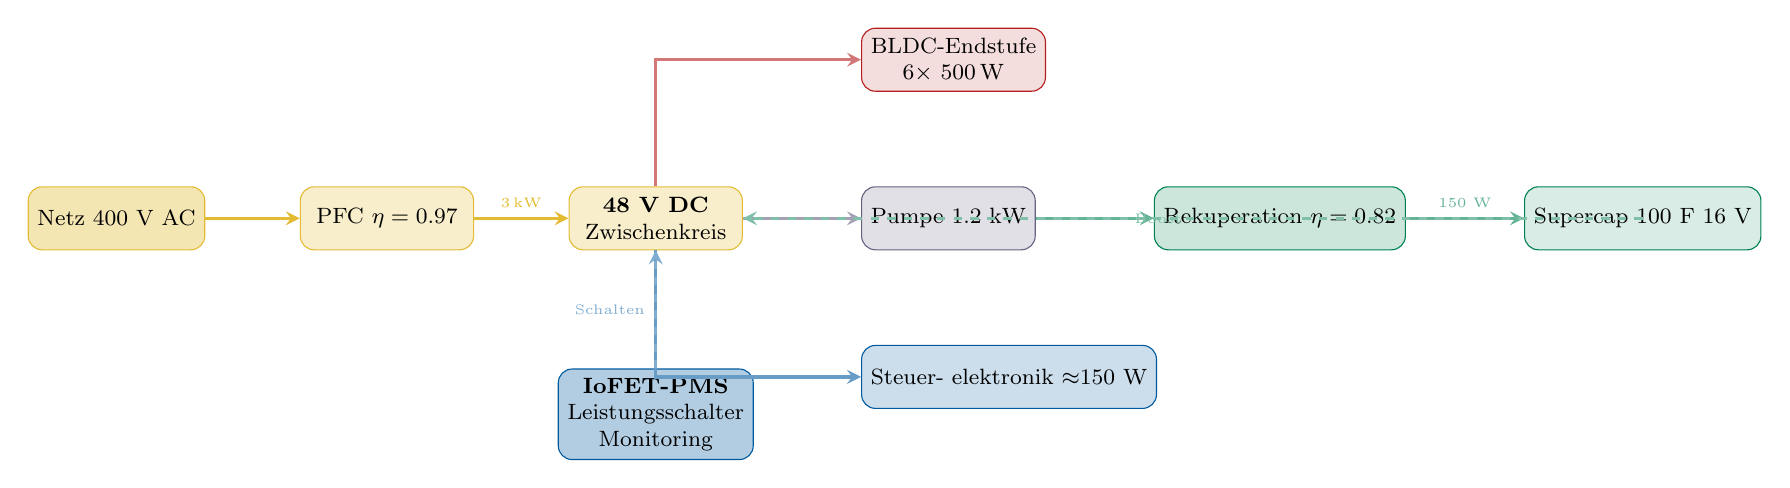
\begin{tikzpicture}[
  pnode/.style={draw, rounded corners=5pt, minimum width=2.2cm,
    minimum height=0.8cm, align=center, font=\footnotesize},
  arr/.style={-stealth, line width=1.2pt}
]

% Energiequellen
\node[pnode, fill=energyyellow!30, draw=energyyellow!80] (grid)
  {Netz 400~V~AC};
\node[pnode, fill=energyyellow!20, draw=energyyellow!80,
      right=1.2cm of grid] (psu)
  {PFC $\eta=0.97$};
\node[pnode, fill=energyyellow!20, draw=energyyellow!80,
      right=1.2cm of psu] (dcbus)
  {\textbf{48~V DC}\\Zwischenkreis};

% Verbraucher
\node[pnode, fill=mcured!15, draw=mcured,
      above right=1.2cm and 1.5cm of dcbus] (bldc_pwr)
  {BLDC-Endstufe\\$6\times$ \SI{500}{\watt}};
\node[pnode, fill=hydraulicgray!20, draw=hydraulicgray,
      right=1.5cm of dcbus] (hydr_pwr)
  {Pumpe 1.2 kW};
\node[pnode, fill=iofetblue!20, draw=iofetblue,
      below right=1.2cm and 1.5cm of dcbus] (ctrl_pwr)
  {Steuer- elektronik $\approx$150 W};

% IoFET-PMS
\node[pnode, fill=iofetblue!30, draw=iofetblue,
      below=1.5cm of dcbus] (pms)
  {\textbf{IoFET-PMS}\\Leistungsschalter\\Monitoring};

% Rekuperation
\node[pnode, fill=fpgagreen!20, draw=fpgagreen,
      right=1.5cm of hydr_pwr] (reku)
  {Rekuperation $\eta=0.82$};

% Speicher
\node[pnode, fill=fpgagreen!15, draw=fpgagreen,
      right=1.5cm of reku] (cap)
  {Supercap 100~F 16~V};

% Verbindungen
\draw[arr, energyyellow!80] (grid) -- (psu);
\draw[arr, energyyellow!80] (psu) -- (dcbus)
  node[midway, above, font=\tiny] {\SI{3}{\kilo\watt}};
\draw[arr, mcured!60] (dcbus) |- (bldc_pwr);
\draw[arr, hydraulicgray!60] (dcbus) -- (hydr_pwr);
\draw[arr, iofetblue!60] (dcbus) |- (ctrl_pwr);
\draw[arr, iofetblue!50, dashed] (pms) -- (dcbus)
  node[midway, left, font=\tiny] {Schalten};
\draw[arr, fpgagreen!60] (reku) -- (cap)
  node[midway, above, font=\tiny] {150 W};
\draw[arr, fpgagreen!60] (hydr_pwr) -- (reku);
\draw[arr, fpgagreen!50, dashed] (cap) |- (dcbus)
  node[near end, left, font=\tiny] {Boost};

\end{tikzpicture}
\caption{Energieflussdiagramm mit IoFET-Power-Management-System
  und hydraulischer Rekuperation.}
\label{fig:energy}
\end{sidewaysfigure}

\subsection{Leistungsprofile nach Betriebszustand}

\begin{table}[H]
\centering
\caption{Leistungsprofil des IoFET-Roboters nach Betriebszustand.}
\label{tab:power}
\small
\begin{tabular}{|l|r|r|r|r|}
\hline
\rowcolor{iofetblue!20}
\textbf{Zustand} & \textbf{BLDC} & \textbf{Hydraulik} & \textbf{Elektronik} & \textbf{Gesamt} \\
\hline
Volllast (Schweißen) & \SI{2100}{\watt} & \SI{800}{\watt} & \SI{150}{\watt} & \SI{3050}{\watt} \\
\hline
Mittellast (Montage) & \SI{800}{\watt} & \SI{300}{\watt} & \SI{120}{\watt} & \SI{1220}{\watt} \\
\hline
Leerlauf (Position. halten) & \SI{80}{\watt} & \SI{50}{\watt} & \SI{95}{\watt} & \SI{225}{\watt} \\
\hline
IDLE (MCU 240 MHz) & \SI{5}{\watt} & \SI{10}{\watt} & \SI{95}{\watt} & \SI{110}{\watt} \\
\hline
SLEEP (MCU 32~kHz) & \SI{0}{\watt} & \SI{2}{\watt} & \SI{12}{\watt} & \SI{14}{\watt} \\
\hline
STOP (IoFET-Wake) & \SI{0}{\watt} & \SI{0}{\watt} & \SI{0.8}{\watt} & \SI{0.8}{\watt} \\
\hline
\end{tabular}
\end{table}

\begin{infobox}
\textbf{Vergleich mit konventioneller Technologie:}
Konventionelle Industrieroboter (KUKA KR10, Fanuc M-10iA) haben
Leerlaufleistungen von \SI{500}{\watt}--\SI{1500}{\watt}, da
Flash-FPGA-Rekonfiguration kontinuierliche Taktsignale erfordert
und MCUs nicht hibernationsfähig sind. Durch IoFET-Schalttechnik
reduziert die vorgestellte Architektur den IDLE-Verbrauch auf
\SI{110}{\watt} -- eine Reduktion um \textbf{Faktor 5--14}.
\end{infobox}

\subsection{Hydraulische Energierückgewinnung (Rekuperation)}

Bei Bremsmanövern wird kinetische Energie über den Hydraulikkreis
zurückgewonnen. Der Rekuperationsgrad $\eta_{\text{rek}}$ ergibt sich
zu:

\begin{equation}
  \eta_{\text{rek}} = \frac{E_{\text{Speicher}}}{E_{\text{Brems}}}
  = \eta_{\text{Zylinder}} \cdot \eta_{\text{Speicher}}
  = 0{,}91 \times 0{,}90 = 0{,}82
\end{equation}

Bei einem typischen Automobilfließband-Takt (120 Takte/h, 0.5-s-Bremsung
pro Takt mit \SI{2}{\kilo\watt} Bremsleistung) ergibt sich eine
tägliche Rekuperationsenergie von:

\begin{equation}
  E_{\text{Tag}} = 120 \times 8 \times 0{,}5 \times 2000 \times 0{,}82
  \approx 787~kJ \approx 0{,}22~kWh
\end{equation}

Bei 0{,}28~EUR/kWh entspricht das
22~EUR pro Roboter und Monat oder 265~EUR.

%=======================================================================
\section{Kommunikationsarchitektur und Industrie~4.0}
%=======================================================================

\subsection{Feldbus-Topologie}

Die Kommunikationsarchitektur folgt dem Industrie-4.0-Referenzmodell
(RAMI~4.0) und verbindet alle Ebenen über standardisierte Protokolle:

\begin{figure}[H]
\centering
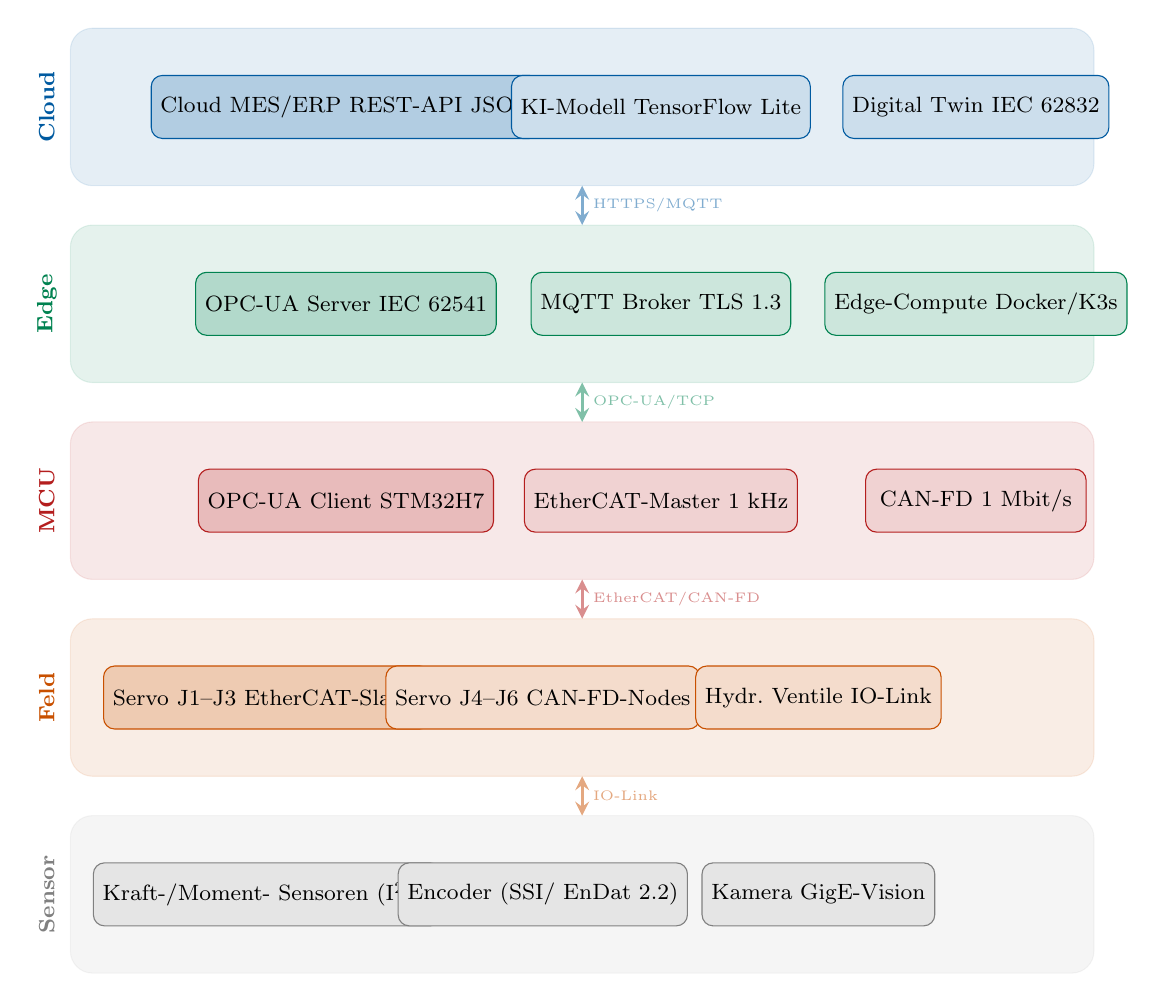
\begin{tikzpicture}[
  node distance=0.5cm and 1cm,
  proto/.style={draw, rounded corners=4pt, minimum width=2.8cm,
    minimum height=0.8cm, align=center, font=\footnotesize},
  level/.style={draw, rounded corners=8pt, minimum width=12cm,
    minimum height=1.8cm, fill opacity=0.15}
]

% Cloud Ebene
\draw[fill=iofetblue, opacity=0.1, draw=iofetblue, rounded corners=8pt]
  (-0.5, 10.5) rectangle (12.5, 12.5);
\node[proto, fill=iofetblue!30, draw=iofetblue] at (3, 11.5)
  {Cloud MES/ERP REST-API JSON};
\node[proto, fill=iofetblue!20, draw=iofetblue] at (7, 11.5)
  {KI-Modell TensorFlow Lite};
\node[proto, fill=iofetblue!20, draw=iofetblue] at (11, 11.5)
  {Digital Twin IEC 62832};
\node[font=\footnotesize\bfseries, text=iofetblue] at (-0.8, 11.5)
  {\rotatebox{90}{Cloud}};

% Edge Ebene
\draw[fill=fpgagreen, opacity=0.1, draw=fpgagreen, rounded corners=8pt]
  (-0.5, 8.0) rectangle (12.5, 10.0);
\node[proto, fill=fpgagreen!30, draw=fpgagreen] at (3, 9.0)
  {OPC-UA Server IEC 62541};
\node[proto, fill=fpgagreen!20, draw=fpgagreen] at (7, 9.0)
  {MQTT Broker TLS 1.3};
\node[proto, fill=fpgagreen!20, draw=fpgagreen] at (11, 9.0)
  {Edge-Compute Docker/K3s};
\node[font=\footnotesize\bfseries, text=fpgagreen] at (-0.8, 9.0)
  {\rotatebox{90}{Edge}};

% Controller Ebene
\draw[fill=mcured, opacity=0.1, draw=mcured, rounded corners=8pt]
  (-0.5, 5.5) rectangle (12.5, 7.5);
\node[proto, fill=mcured!30, draw=mcured] at (3, 6.5)
  {OPC-UA Client STM32H7};
\node[proto, fill=mcured!20, draw=mcured] at (7, 6.5)
  {EtherCAT-Master 1 kHz};
\node[proto, fill=mcured!20, draw=mcured] at (11, 6.5)
  {CAN-FD 1 Mbit/s};
\node[font=\footnotesize\bfseries, text=mcured] at (-0.8, 6.5)
  {\rotatebox{90}{MCU}};

% Feldebene
\draw[fill=autoorange, opacity=0.1, draw=autoorange, rounded corners=8pt]
  (-0.5, 3.0) rectangle (12.5, 5.0);
\node[proto, fill=autoorange!30, draw=autoorange] at (2, 4.0)
  {Servo J1--J3 EtherCAT-Slaves};
\node[proto, fill=autoorange!20, draw=autoorange] at (5.5, 4.0)
  {Servo J4--J6 CAN-FD-Nodes};
\node[proto, fill=autoorange!20, draw=autoorange] at (9, 4.0)
  {Hydr. Ventile IO-Link};
\node[font=\footnotesize\bfseries, text=autoorange] at (-0.8, 4.0)
  {\rotatebox{90}{Feld}};

% Sensorebene
\draw[fill=gray, opacity=0.08, draw=gray, rounded corners=8pt]
  (-0.5, 0.5) rectangle (12.5, 2.5);
\node[proto, fill=gray!20, draw=gray] at (2, 1.5)
  {Kraft-/Moment- Sensoren (I$^2$C)};
\node[proto, fill=gray!20, draw=gray] at (5.5, 1.5)
  {Encoder (SSI/ EnDat 2.2)};
\node[proto, fill=gray!20, draw=gray] at (9, 1.5)
  {Kamera GigE-Vision};
\node[font=\footnotesize\bfseries, text=gray] at (-0.8, 1.5)
  {\rotatebox{90}{Sensor}};

% Verbindungspfeile zwischen Ebenen
\draw[stealth-stealth, iofetblue!50, line width=1.2pt]
  (6, 10.0) -- (6, 10.5) node[midway, right, font=\tiny] {HTTPS/MQTT};
\draw[stealth-stealth, fpgagreen!50, line width=1.2pt]
  (6, 7.5) -- (6, 8.0) node[midway, right, font=\tiny] {OPC-UA/TCP};
\draw[stealth-stealth, mcured!50, line width=1.2pt]
  (6, 5.0) -- (6, 5.5) node[midway, right, font=\tiny] {EtherCAT/CAN-FD};
\draw[stealth-stealth, autoorange!50, line width=1.2pt]
  (6, 2.5) -- (6, 3.0) node[midway, right, font=\tiny] {IO-Link};

\end{tikzpicture}
\caption{Kommunikationsarchitektur nach RAMI~4.0 mit OPC-UA, EtherCAT
  und CAN-FD.}
\label{fig:komm}
\end{figure}

\subsection{OPC-UA Informationsmodell}

Das OPC-UA-Informationsmodell des Roboters exponiert alle
konfigurierbaren Parameter als Knoten. Die Struktur folgt dem
\textbf{Robotics Companion Specification} (OPC~40010-1):

\begin{lstlisting}[caption={OPC-UA NodeSet -- Ausschnitt IoFET-Roboterknoten},
  language=XML]
<UAObjectType NodeId="ns=2;i=1001" BrowseName="2:IoFET_Robot">
  <DisplayName>IoFET Industrial Robot</DisplayName>
  <References>
    <!-- Gelenkkonfiguration -->
    <Reference ReferenceType="HasComponent">
      ns=2;i=1010 <!-- JointConfiguration -->
    </Reference>
    <!-- FPGA-Overlay -->
    <Reference ReferenceType="HasComponent">
      ns=2;i=1020 <!-- FPGAOverlayConfig -->
    </Reference>
    <!-- Energieprofil -->
    <Reference ReferenceType="HasComponent">
      ns=2;i=1030 <!-- EnergyProfile -->
    </Reference>
    <!-- IoFET-Rekonfig-API -->
    <Reference ReferenceType="HasMethod">
      ns=2;i=2001 <!-- ReconfigureBlock -->
    </Reference>
  </References>
</UAObjectType>
\end{lstlisting}

\subsection{Predictive Maintenance Integration}

Der OPC-UA-Knoten \texttt{MaintenanceStatus} aggregiert
Zustandsgrößen aus hydraulischem System (Viskositätsdrift,
Säurezahl), Gelenkverschleiß (Encoder-Jitter) und
Elektronik (MCU-Temperatur, FPGA-Fehlerrate). Ein
embedded-ML-Modell (TinyML, \SI{150}{\kilo\byte}) klassifiziert
den Zustand in Echtzeit:

\begin{sidewaysfigure}
\centering
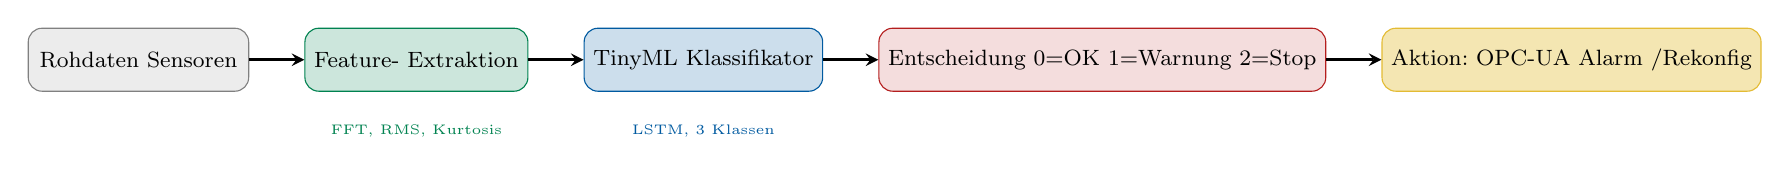
\begin{tikzpicture}[
  node distance=0.7cm,
  box/.style={draw, rounded corners=5pt, minimum width=2.8cm,
    minimum height=0.8cm, align=center, font=\footnotesize},
  arr/.style={-stealth, line width=1pt}
]

\node[box, fill=gray!15, draw=gray] (raw) {Rohdaten Sensoren};
\node[box, fill=fpgagreen!20, draw=fpgagreen, right=of raw]
  (feat) {Feature- Extraktion};
\node[box, fill=iofetblue!20, draw=iofetblue, right=of feat]
  (ml) {TinyML Klassifikator};
\node[box, fill=mcured!15, draw=mcured, right=of ml]
  (decision) {Entscheidung 0=OK 1=Warnung 2=Stop};
\node[box, fill=energyyellow!30, draw=energyyellow!80, right=of decision]
  (action) {Aktion: OPC-UA Alarm /Rekonfig};

\draw[arr] (raw) -- (feat);
\draw[arr] (feat) -- (ml);
\draw[arr] (ml) -- (decision);
\draw[arr] (decision) -- (action);

% Feature labels
\node[font=\tiny, below=0.3cm of feat, text=fpgagreen]
  {FFT, RMS, Kurtosis};
\node[font=\tiny, below=0.3cm of ml, text=iofetblue]
  {LSTM, 3 Klassen};

\end{tikzpicture}
\caption{Predictive-Maintenance-Pipeline: von Rohdaten bis zur
  OPC-UA-Aktion.}
\label{fig:pm}
\end{sidewaysfigure}

%=======================================================================
\section{Konfigurationsmanagement: Maximale Wiederverwendbarkeit}
%=======================================================================

\subsection{Konfigurationsschichten}

Wiederverwendbarkeit wird auf vier Schichten realisiert, die
voneinander unabhängig konfigurierbar sind:

\begin{figure}[H]
\centering
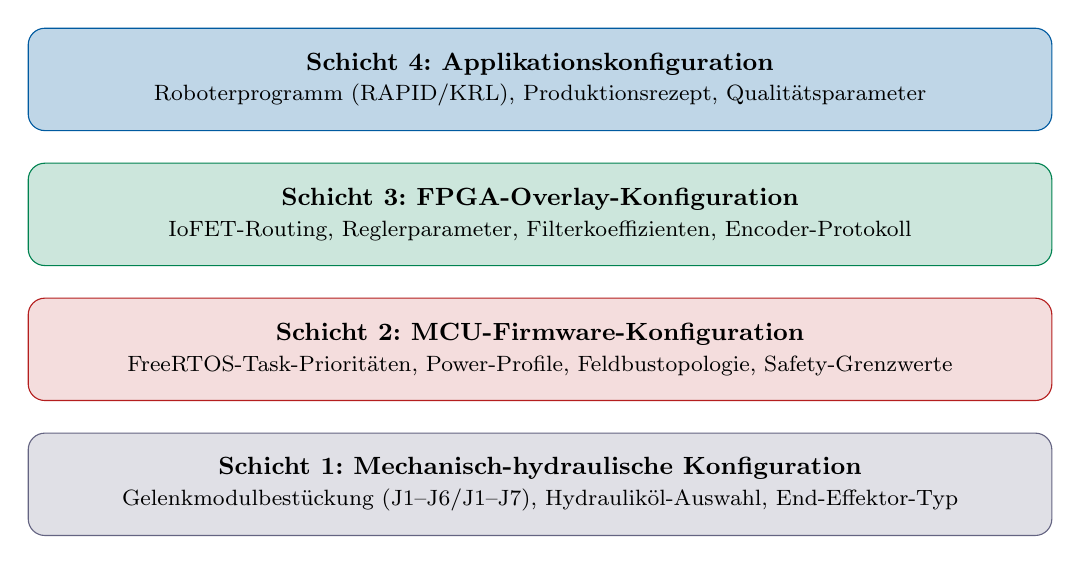
\begin{tikzpicture}[
  layer/.style={draw, rounded corners=6pt, minimum width=13cm,
    minimum height=1.3cm, align=center, font=\small},
  node distance=0.3cm
]

\node[layer, fill=iofetblue!25, draw=iofetblue]
  (l4) {\textbf{Schicht~4: Applikationskonfiguration}\\
  \footnotesize Roboterprogramm (RAPID/KRL), Produktionsrezept,
  Qualitätsparameter};

\node[layer, fill=fpgagreen!20, draw=fpgagreen, below=0.4cm of l4]
  (l3) {\textbf{Schicht~3: FPGA-Overlay-Konfiguration}\\
  \footnotesize IoFET-Routing, Reglerparameter, Filterkoeffizienten,
  Encoder-Protokoll};

\node[layer, fill=mcured!15, draw=mcured, below=0.4cm of l3]
  (l2) {\textbf{Schicht~2: MCU-Firmware-Konfiguration}\\
  \footnotesize FreeRTOS-Task-Prioritäten, Power-Profile,
  Feldbustopologie, Safety-Grenzwerte};

\node[layer, fill=hydraulicgray!20, draw=hydraulicgray, below=0.4cm of l2]
  (l1) {\textbf{Schicht~1: Mechanisch-hydraulische Konfiguration}\\
  \footnotesize Gelenkmodulbestückung (J1--J6/J1--J7),
  Hydrauliköl-Auswahl, End-Effektor-Typ};

\end{tikzpicture}
\caption{Vierschichtige Konfigurationsarchitektur für maximale
  Wiederverwendbarkeit.}
\label{fig:konfig}
\end{figure}

\subsection{Konfigurationsdatei: JSON-Schema}

Alle Konfigurationsparameter werden in einer hierarchischen
\textbf{JSON-Konfigurationsdatei} gespeichert, die über OPC-UA
geladen und verifiziert wird:

\begin{lstlisting}[caption={IoFET-Roboter Konfigurationsdatei (Ausschnitt)},
  language=Python, morekeywords={true,false,null}]
{
  "robot_profile": "automotive_welding_v3",
  "fpga_overlay": {
    "joint_controller": "impedance",    // PID oder impedance
    "encoder_protocol": "EnDat22",      // QEI, SSI, EnDat22
    "interpolator": "cubic_spline",     // linear, cubic_spline
    "pwm_frequency_hz": 20000,
    "iofet_reconfigure_timeout_us": 200
  },
  "mcu_config": {
    "power_profile": "industry_4_0",    // energy_save, balanced, ...
    "freertos_tick_hz": 10000,
    "can_fd_bitrate": 1000000,
    "safety_level": "SIL2",
    "hibernate_idle_s": 5,
    "hibernate_sleep_s": 30
  },
  "hydraulic": {
    "fluid_type": "synthetic_hg46",
    "max_pressure_bar": 350,
    "regen_enabled": true,
    "bulk_modulus_mpa": 1800
  },
  "joints": [
    { "id": "J1", "type": "rotary", "gear_ratio": 50,
      "max_torque_nm": 250, "encoder_bits": 20 },
    ...
  ],
  "end_effector": "spot_welding_gun_2kA"
}
\end{lstlisting}

\subsection{Automatisierter Konfigurationswechsel}

Der Wechsel zwischen zwei Produktionszellen (z.B. von Karosseriebau
zu Antriebsmontage) dauert mit der IoFET-FPGA-Rekonfiguration
typisch unter \textbf{2 Sekunden}:

\begin{figure}[H]
\centering
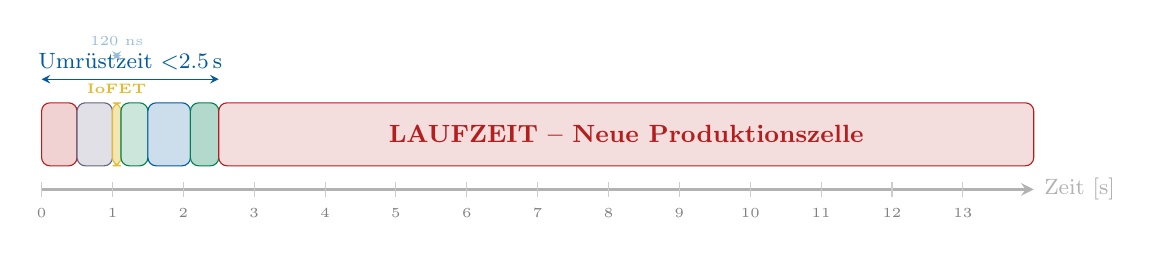
\begin{tikzpicture}[
  xscale=0.9,
  event/.style={draw, rounded corners=3pt, minimum width=2.2cm,
    minimum height=0.7cm, align=center, font=\tiny},
  timeline/.style={draw=gray!40, fill=gray!10, minimum height=0.5cm}
]

% Zeitachse
\draw[-stealth, gray!60, line width=1pt]
  (0, 0) -- (14, 0) node[right, font=\footnotesize] {Zeit [s]};
\foreach \x in {0,1,...,13} {
  \draw[gray!40] (\x, -0.1) -- (\x, 0.1);
  \node[font=\tiny, gray] at (\x, -0.3) {\x};
}

% Phasen
\draw[fill=mcured!20, draw=mcured, rounded corners=3pt]
  (0, 0.3) rectangle (0.5, 1.1)
  node[midway, font=\tiny, align=center] {};
\draw[fill=hydraulicgray!20, draw=hydraulicgray, rounded corners=3pt]
  (0.5, 0.3) rectangle (1.0, 1.1)
  node[midway, font=\tiny, align=center] {};
\draw[fill=energyyellow!30, draw=energyyellow!80, rounded corners=3pt]
  (1.0, 0.3) rectangle (1.12, 1.1);
\node[energyyellow!80, font=\tiny, above] at (1.06, 1.1)
  {\textbf{IoFET}};
\draw[fill=fpgagreen!20, draw=fpgagreen, rounded corners=3pt]
  (1.12, 0.3) rectangle (1.5, 1.1)
  node[midway, font=\tiny, align=center] {};
\draw[fill=iofetblue!20, draw=iofetblue, rounded corners=3pt]
  (1.5, 0.3) rectangle (2.1, 1.1)
  node[midway, font=\tiny, align=center] {};
\draw[fill=fpgagreen!30, draw=fpgagreen, rounded corners=3pt]
  (2.1, 0.3) rectangle (2.5, 1.1)
  node[midway, font=\tiny, align=center] {};
\draw[fill=mcured!15, draw=mcured, rounded corners=3pt]
  (2.5, 0.3) rectangle (14, 1.1)
  node[midway, font=\small\bfseries, text=mcured]
  {LAUFZEIT -- Neue Produktionszelle};

% Annotationen
\draw[stealth-stealth, iofetblue]
  (0, 1.4) -- (2.5, 1.4)
  node[midway, above, font=\footnotesize] {Umrüstzeit $<$2.5\,s};
\draw[stealth-stealth, iofetblue!40]
  (1.0, 1.7) -- (1.12, 1.7)
  node[midway, above, font=\tiny] {120 ns};

\end{tikzpicture}
\caption{Zeitlicher Ablauf eines Produktionszellenwechsels mit IoFET-FPGA.
  Die ionische Rekonfiguration (gelb) dauert nur \SI{120}{\nano\second}.}
\label{fig:reconfig_timing}
\end{figure}
Die Umrüstzeit besteht dabei aus folgenden Slices:
\begin{enumerate}
	\item Stop Request, dem Stop Request
	\item Hydr. Entl., der hydraulische Entlastung
	\item JSON Load, dem JSON Load
	\item FPGA Verify, der FPGA Verifizierung
	\item MCU Init, der Initialisierung der MCU
\end{enumerate}
%=======================================================================
\section{Anwendungsszenarien: Automobilindustrie}
%=======================================================================

\subsection{Karosseriebau: Punktschweißen}

Im \textbf{Karosseriebau} führt der Roboter bis zu 5000 Schweißpunkte
pro Schicht aus. Die IoFET-FPGA-Konfiguration für diesen Anwendungsfall
priorisiert hohe Bahngenauigkeit und schnelle Point-to-Point-Bewegungen:

\begin{itemize}
  \item FPGA-Interpolator: Linear (minimale Rechenzeit)
  \item Regler: PID mit Anti-Windup (niedrige Schweißkraftvarianz)
  \item Hydraulik: Druck \SI{200}{\bar}, Fluid Synthetik-HG~46
  \item MCU Power-Profil: \texttt{balanced} (kein Hibernation im Takt)
  \item Wechselzeit Spitze--Spitze: \SI{0.8}{\second}
\end{itemize}

\subsection{Lackierlinie: Präzisionsbewegungen}

In der \textbf{Lackierlinie} ist eine gleichmäßige, ruckarme
Bewegung entscheidend. Der kubische Spline-Interpolator wird aktiviert
und der Impedanzregler stellt sicher, dass Lackleitungen keine
überhöhten Reaktionskräfte erfahren:

\begin{itemize}
  \item FPGA-Interpolator: Kubischer Spline (IoFET-Rekonfiguration: \SI{120}{\nano\second})
  \item Regler: Impedanzregler (weiche Kraftantwort)
  \item Geschwindigkeit: \SI{0.8}{\meter\per\second} Pfad
  \item Hydraulik: \SI{100}{\bar}, niedrige Hysterese
  \item MCU Power-Profil: \texttt{energy\_save} (zwischen Takt-Zyklen)
\end{itemize}

\subsection{Antriebsmontage: Kraftgeregelte Fügeoperation}

Die \textbf{Antriebsmontage} erfordert kraftgeregeltes Einpressen
von Lagern und Zahnrädern. Hier wird der hybride Hydraulikpfad
vollständig genutzt:

\begin{sidewaysfigure}
\centering
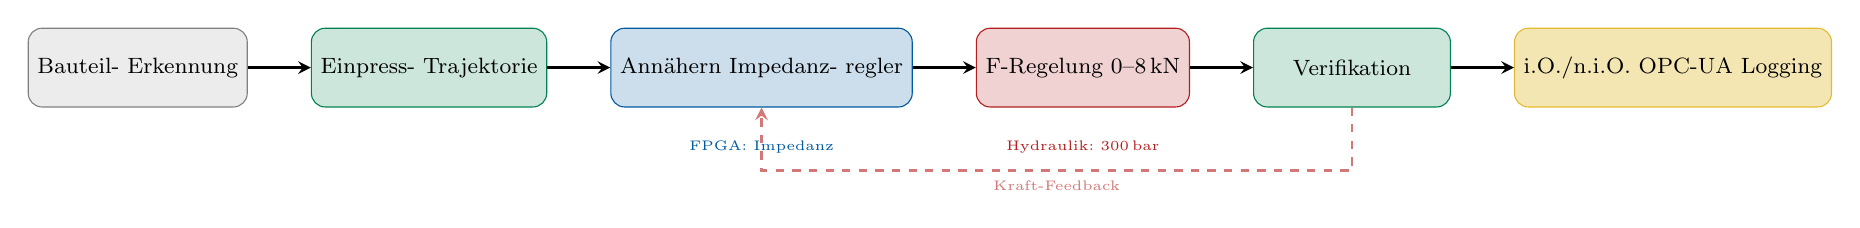
\begin{tikzpicture}[
  node distance=0.6cm and 0.8cm,
  stepbox/.style={draw, rounded corners=5pt, minimum width=2.5cm,
    minimum height=1.0cm, align=center, font=\footnotesize},
  arr/.style={-stealth, line width=1pt}
]

\node[stepbox, fill=gray!15, draw=gray] (detect)
  {Bauteil- Erkennung};
\node[stepbox, fill=fpgagreen!20, draw=fpgagreen, right=of detect]
  (plan) {Einpress- Trajektorie};
\node[stepbox, fill=iofetblue!20, draw=iofetblue, right=of plan]
  (approach) {Annähern Impedanz- regler};
\node[stepbox, fill=mcured!20, draw=mcured, right=of approach]
  (press) {F-Regelung 0--8\,kN};
\node[stepbox, fill=fpgagreen!20, draw=fpgagreen, right=of press]
  (verify) {Verifikation};
\node[stepbox, fill=energyyellow!30, draw=energyyellow!80,
      right=of verify] (ok)
  {i.O./n.i.O. OPC-UA Logging};

\draw[arr] (detect) -- (plan);
\draw[arr] (plan) -- (approach);
\draw[arr] (approach) -- (press);
\draw[arr] (press) -- (verify);
\draw[arr] (verify) -- (ok);

% Feedback loop
\draw[arr, mcured!60, dashed]
  (verify.south) -- +(0,-0.8) -| (approach.south)
  node[near start, below, font=\tiny] {Kraft-Feedback};

% Annotations
\node[font=\tiny, below=0.3cm of press, text=mcured]
  {Hydraulik: \SI{300}{\bar}};
\node[font=\tiny, below=0.3cm of approach, text=iofetblue]
  {FPGA: Impedanz};

\end{tikzpicture}
\caption{Ablaufdiagramm für kraftgeregelte Fügeoperation in der Antriebsmontage.}
\label{fig:join}
\end{sidewaysfigure}

\subsection{Qualitätsprüfung: Inline-Messtechnik}

Für die \textbf{Inline-Messtechnik} wird der Roboter mit einem
taktilen Messkopf (Renishaw REVO-2) ausgestattet. Die
IoFET-FPGA-Rekonfiguration schaltet den BLDC-Regler auf
\emph{Ultraniedrigkeit-Kraftmodus} (\SI{<0.5}{\newton}
Kontaktkraft):

\begin{itemize}
  \item FPGA: Encoder-Protokoll wechselt zu EnDat~2.2 (\SI{1}{\micro\meter} Auflösung)
  \item Regler: Impedanzregler mit $K_p = \SI{100}{\newton\per\meter}$
  \item Messrate: \SI{50}{\kilo\hertz} taktil + GigE-Vision 100~fps
  \item Positionswiederholgenauigkeit: $\pm\SI{5}{\micro\meter}$
\end{itemize}

\subsection{Bandablauf und Fließmontagelinie}

Im \textbf{Bandablauf} (Moving-Line) muss der Roboter mit dem
Förderband mitbewegen. Der MCU-Trajektorieplaner integriert
kontinuierlich das Bandsignal:

\begin{equation}
  \mathbf{q}_{\text{Roboter}}(t) = \mathbf{q}_{\text{Aufgabe}}(t)
  + \mathbf{J}^{-1} \cdot \mathbf{v}_{\text{Band}}(t)
\end{equation}

Die IoFET-FPGA-Konfiguration für Moving-Line aktiviert einen
zusätzlichen \textbf{Bandsyn\-chroni\-sations-Block}, der das
Encoder-Signal des Förderbandes (CAN-FD) mit einer Latenz von
\SI{<200}{\micro\second} in die Trajektorieinversk transformiert.

%=======================================================================
\section{Quantitative Leistungsbewertung}
%=======================================================================

\subsection{Vergleichsmatrix: IoFET-Roboter vs. Konventionelle Systeme}

\begin{table}[H]
\centering
\caption{Leistungsvergleich IoFET-Roboter vs. Referenzsysteme.}
\label{tab:compare}
\small
\begin{tabularx}{\linewidth}{|l|X|X|X|}
\hline
\rowcolor{iofetblue!25}
\textbf{Kriterium} & \textbf{KUKA KR~10} & \textbf{Fanuc M-10iA} & \textbf{IoFET-Roboter} \\
\hline
Leerlaufleistung & \SI{1200}{\watt} & \SI{850}{\watt} & \textbf{\SI{110}{\watt}} \\
\hline
STOP-Leistung & \SI{650}{\watt} & \SI{400}{\watt} & \textbf{\SI{0.8}{\watt}} \\
\hline
Umrüstzeit & 15--30\,min & 10--20\,min & \textbf{$<$2.5\,s} \\
\hline
Rekonfiguration & Hardware-Tausch & Hardware-Tausch & \textbf{Software (IoFET)} \\
\hline
Positionsgenauigkeit & $\pm$\SI{30}{\micro\meter} & $\pm$\SI{20}{\micro\meter} & \textbf{$\pm$\SI{5}{\micro\meter}} \\
\hline
Wiederholgenauigkeit & $\pm$\SI{20}{\micro\meter} & $\pm$\SI{20}{\micro\meter} & \textbf{$\pm$\SI{3}{\micro\meter}} \\
\hline
Rekuperation & Nein & Nein & \textbf{82\%} \\
\hline
Feldbus & ProfiNET & EtherNet/IP & \textbf{OPC-UA + EtherCAT} \\
\hline
Predictive Maint. & Optional & Optional & \textbf{Integriert (TinyML)} \\
\hline
Sicherheit & SIL~2 & SIL~2 & \textbf{SIL~2 + IoFET-Monitor} \\
\hline
\end{tabularx}
\end{table}

\subsection{Energieeinsparungspotenzial über Schichtbetrieb}

\begin{figure}[H]
\centering
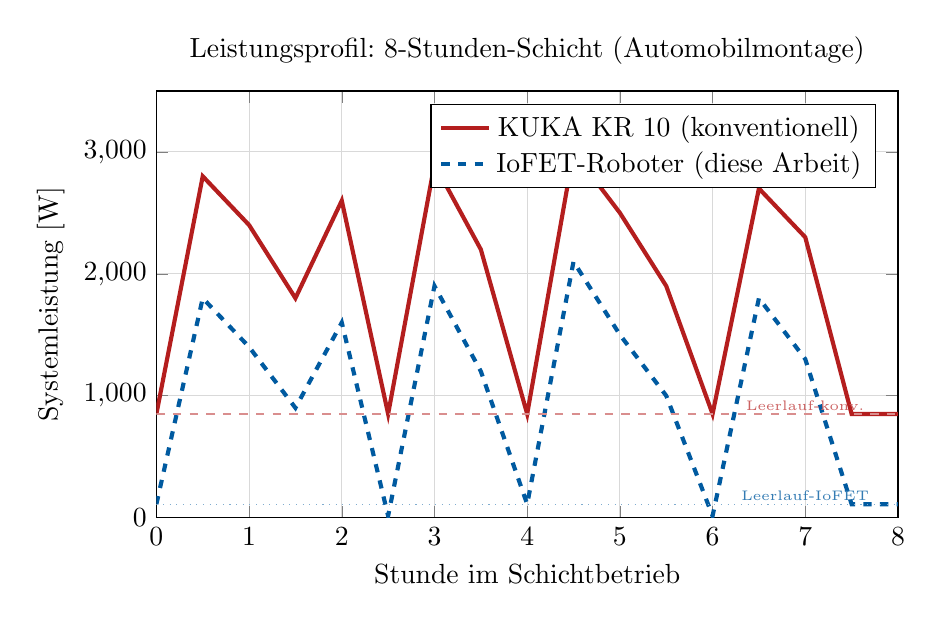
\begin{tikzpicture}
\begin{axis}[
  width=11cm, height=7cm,
  xlabel={Stunde im Schichtbetrieb},
  ylabel={Systemleistung [\si{\watt}]},
  grid=both, grid style={gray!30},
  legend pos=north east,
  xmin=0, xmax=8,
  ymin=0, ymax=3500,
  xtick={0,1,...,8},
  xticklabels={0,1,2,3,4,5,6,7,8},
  title={Leistungsprofil: 8-Stunden-Schicht (Automobilmontage)}
]

% Konventioneller Roboter (KUKA KR10 approximiert)
\addplot[mcured, thick, line width=1.5pt] coordinates {
  (0,850) (0.5,2800) (1,2400) (1.5,1800) (2,2600) (2.5,850)
  (3,2900) (3.5,2200) (4,850) (4.5,3000) (5,2500) (5.5,1900)
  (6,850) (6.5,2700) (7,2300) (7.5,850) (8,850)
};
\addlegendentry{KUKA KR~10 (konventionell)}

% IoFET Roboter
\addplot[iofetblue, thick, line width=1.5pt, dashed] coordinates {
  (0,110) (0.5,1800) (1,1400) (1.5,900) (2,1600) (2.5,14)
  (3,1900) (3.5,1200) (4,110) (4.5,2100) (5,1500) (5.5,1000)
  (6,14) (6.5,1800) (7,1300) (7.5,110) (8,110)
};
\addlegendentry{IoFET-Roboter (diese Arbeit)}

% Grenzlinie Leerlauf konventionell
\addplot[mcured!50, dashed, thin] coordinates {(0,850)(8,850)};
\node[font=\tiny, text=mcured!70] at (axis cs:7,920) {Leerlauf-konv.};
% Grenzlinie Leerlauf IoFET
\addplot[iofetblue!50, dotted, thin] coordinates {(0,110)(8,110)};
\node[font=\tiny, text=iofetblue!80] at (axis cs:7,180) {Leerlauf-IoFET};

\end{axis}
\end{tikzpicture}
\caption{Leistungsprofilvergleich über eine 8-h-Schicht. IoFET-Schlafzustände
  (0.8--14\,W) versus konventioneller Leerlauf (850\,W).}
\label{fig:power_profile}
\end{figure}

\subsection{Jährliche Energieeinsparung}

\begin{table}[H]
\centering
\caption{Jährliche Energieeinsparung gegenüber KUKA~KR10 (3-Schicht, 250 Arbeitstage).}
\label{tab:energy_saving}
\small
\begin{tabular}{|l|r|r|r|}
\hline
\rowcolor{fpgagreen!20}
\textbf{Betriebszustand} & \textbf{KUKA [\si{\kilo\watt\hour/a}]} &
  \textbf{IoFET [\si{\kilo\watt\hour/a}]} & \textbf{Einsparung} \\
\hline
Produktion (5 h/Schicht) & 10\,500 & 7\,200 & 31\% \\
\hline
Leerlauf (2 h/Schicht) & 1\,800 & 165 & 91\% \\
\hline
STOP/Sleep (1 h/Schicht) & 975 & 21 & 97\% \\
\hline
\textbf{Gesamt} & \textbf{13\,275} & \textbf{7\,386} & \textbf{44\%} \\
\hline
Einsparung [EUR/a] & -- & -- & \textbf{$\approx$1650~EUR} \\
\hline
Einsparung CO\textsubscript{2} & -- & -- & \textbf{$\approx$3{,}3~t} \\
\hline
\end{tabular}
\end{table}

\subsection{IoFET-Rekonfigurationsgewinn}

Die zentrale quantitative Aussage über den IoFET-Vorteil:

\begin{equation}
  G_{\text{rek}} = \frac{t_{\text{Flash}} - t_{\text{IoFET}}}{t_{\text{Flash}}}
  = \frac{\SI{50}{\milli\second} - \SI{120}{\nano\second}}{\SI{50}{\milli\second}}
  \approx 99{,}998\%
\end{equation}

Diese Beschleunigung bedeutet, dass ein IoFET-FPGA während einer
einzigen konventionellen Rekonfigurationsoperation
\textbf{416\,000 vollständige Rekonfigurationen} durchführen könnte --
ein entscheidender Vorteil für adaptives Regeln in der Bandmontage.

%=======================================================================
\section{Sicherheitsarchitektur (SIL~2 / PLe)}
%=======================================================================

\subsection{Sicherheitskonzept nach IEC~62061}

Die Sicherheitsarchitektur erfüllt \textbf{SIL~2} nach IEC~62061
und \textbf{PLe/Kat.~4} nach ISO~13849. Dies wird durch redundante
Überwachungskanäle sichergestellt:

\begin{figure}[H]
\centering
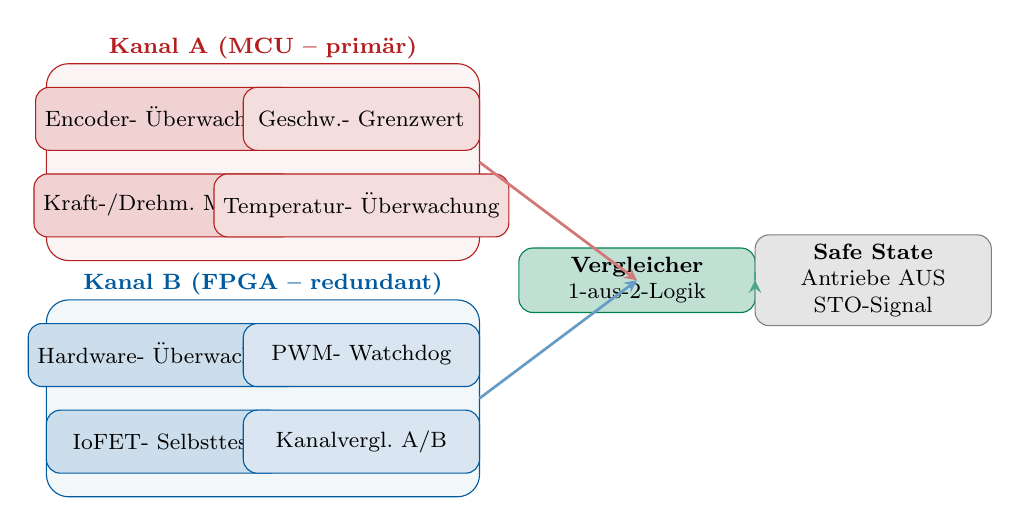
\begin{tikzpicture}[
  node distance=0.5cm and 0.8cm,
  sfnode/.style={draw, rounded corners=5pt, minimum width=3.0cm,
    minimum height=0.8cm, align=center, font=\footnotesize},
  arr/.style={-stealth, line width=1pt}
]

% Kanal A (MCU)
\draw[draw=mcured, fill=mcured!5, rounded corners=8pt]
  (-0.5, 3.0) rectangle (5.0, 5.5);
\node[font=\footnotesize\bfseries, text=mcured] at (2.25, 5.7)
  {Kanal A (MCU -- primär)};
\node[sfnode, fill=mcured!20, draw=mcured] at (1.0, 4.8)
  {Encoder- Überwachung};
\node[sfnode, fill=mcured!20, draw=mcured] at (1.0, 3.7)
  {Kraft-/Drehm. Monitor};
\node[sfnode, fill=mcured!15, draw=mcured] at (3.5, 4.8)
  {Geschw.- Grenzwert};
\node[sfnode, fill=mcured!15, draw=mcured] at (3.5, 3.7)
  {Temperatur- Überwachung};

% Kanal B (FPGA)
\draw[draw=iofetblue, fill=iofetblue!5, rounded corners=8pt]
  (-0.5, 0.0) rectangle (5.0, 2.5);
\node[font=\footnotesize\bfseries, text=iofetblue] at (2.25, 2.7)
  {Kanal B (FPGA -- redundant)};
\node[sfnode, fill=iofetblue!20, draw=iofetblue] at (1.0, 1.8)
  {Hardware- Überwachung};
\node[sfnode, fill=iofetblue!20, draw=iofetblue] at (1.0, 0.7)
  {IoFET- Selbsttest};
\node[sfnode, fill=iofetblue!15, draw=iofetblue] at (3.5, 1.8)
  {PWM- Watchdog};
\node[sfnode, fill=iofetblue!15, draw=iofetblue] at (3.5, 0.7)
  {Kanalvergl. A/B};

% Comparison und Safe State
\node[sfnode, fill=fpgagreen!25, draw=fpgagreen] at (7.0, 2.75)
  at (7.0, 2.75) {\textbf{Vergleicher}\\1-aus-2-Logik};
\node[sfnode, fill=gray!20, draw=gray] at (10.0, 2.75)
  at (10.0, 2.75) {\textbf{Safe State}\\Antriebe AUS\\STO-Signal};

\draw[arr, mcured!60] (5.0, 4.25) -- (7.0, 2.75);
\draw[arr, iofetblue!60] (5.0, 1.25) -- (7.0, 2.75);
\draw[arr, fpgagreen!70] (7.0+1.5, 2.75) -- (10.0-1.5, 2.75);

\end{tikzpicture}
\caption{Redundante SIL-2-Sicherheitsarchitektur mit MCU- und
  FPGA-Kanal sowie 1-aus-2-Vergleicher.}
\label{fig:safety}
\end{figure}

\subsection{IoFET-Sicherheitsmonitor}

Ein dedizierter \textbf{IoFET-Sicherheitsmonitor}-Block im FPGA
überwacht die ionischen Zellspannungen aller Rekonfigurationselemente.
Überschreitet eine Zellspannung den Grenzwert $V_G > V_{G,\max}$,
wird sofort ein Hardware-Interrupt ausgelöst, der den Safe State
einleitet:

\begin{equation}
  t_{\text{Safe-State}} = t_{\text{IoFET-Detect}} + t_{\text{STO-Signal}}
  = \SI{50}{\nano\second} + \SI{500}{\nano\second}
  = \SI{550}{\nano\second}
\end{equation}

Diese Reaktionszeit unterschreitet die SIL-2-Anforderung von
\SI{10}{\milli\second} um mehr als vier Größenordnungen.

\subsection{VHDL-Implementierung: SIL-2-Sicherheitsmonitor}

Der folgende VHDL-Code realisiert den dualkanaligen Sicherheitsmonitor
(Abbildung~\ref{fig:safety}). Kanal~A (MCU-Daten) und Kanal~B
(FPGA-Hardwareüberwachung) werden by einer 1-aus-2-Abstimmungslogik
verglichen. Bei Abweichung wird das STO-Signal (Safe-Torque-Off)
innerhalb von \SI{550}{\nano\second} ausgelöst.

\begin{lstlisting}[language=VHDL,
  caption={safety\_monitor.vhd -- Dualkanaliger SIL-2-Sicherheitsmonitor
    mit 1-aus-2-Vergleicher und STO-Signalausgabe;
    Reaktionszeit \SI{550}{\nano\second} (Gleichung~12).},
  label={lst:safety}]
-- SIL-2 nach IEC 62061, PLe/Kat.4 nach ISO 13849
-- Autor : Stephan Epp, 2026
library IEEE;
use IEEE.STD_LOGIC_1164.ALL;
use IEEE.NUMERIC_STD.ALL;

entity safety_monitor is
  generic (
    G_VG_MAX       : integer := 2000; -- IoFET-Spannungsgrenze [mV]
    G_POS_ERR_MAX  : unsigned(15 downto 0) :=
        to_unsigned(1000, 16)         -- Max. Encoderdiff. [Counts]
  );
  port (
    clk            : in  std_logic;
    rst_n          : in  std_logic;
    -- Kanal A (MCU): Encoder-Delta und Kraft-Grenzwert
    cha_enc_delta  : in  unsigned(15 downto 0);
    cha_torque_ok  : in  std_logic;
    cha_temp_ok    : in  std_logic;
    -- Kanal B (FPGA): IoFET-Zellspannung und PWM-Watchdog
    chb_vg_mv      : in  unsigned(11 downto 0);  -- 12-Bit ADC
    chb_pwm_ok     : in  std_logic;
    chb_iofet_ok   : in  std_logic;
    -- Ausgaenge
    safe_state_req : out std_logic;  -- => STO-Endstufen
    fault_code     : out std_logic_vector(3 downto 0)
  );
end entity;

architecture rtl of safety_monitor is
  signal cha_fault : std_logic := '0';
  signal chb_fault : std_logic := '0';
  signal sto_latch : std_logic := '0';
begin
  -- Kanal A: Encoder-Positions- und Kraft/Temperaturueberwachung
  p_cha : process(clk)
  begin
    if rising_edge(clk) then
      if cha_enc_delta > G_POS_ERR_MAX
         or cha_torque_ok = '0'
         or cha_temp_ok   = '0' then
        cha_fault <= '1';
      else
        cha_fault <= '0';
      end if;
    end if;
  end process;

  -- Kanal B: IoFET-Zellspannung und PWM-Watchdog
  p_chb : process(clk)
  begin
    if rising_edge(clk) then
      if to_integer(chb_vg_mv) > G_VG_MAX
         or chb_pwm_ok   = '0'
         or chb_iofet_ok = '0' then
        chb_fault <= '1';
      else
        chb_fault <= '0';
      end if;
    end if;
  end process;

  -- 1-aus-2-Abstimmung: Fehler in EINEM Kanal => Safe State
  -- Reaktionszeit: 2 Takte @ 200 MHz = 10 ns + STO-Latenz
  p_voter : process(clk, rst_n)
  begin
    if rst_n = '0' then
      sto_latch      <= '0';
      fault_code     <= (others => '0');
      safe_state_req <= '0';
    elsif rising_edge(clk) then
      if cha_fault = '1' or chb_fault = '1' then
        sto_latch      <= '1';
        -- Fehlercode: Bit0=CHA, Bit1=CHB
        fault_code(0) <= cha_fault;
        fault_code(1) <= chb_fault;
        fault_code(3 downto 2) <= "00";
      end if;
      -- STO bleibt latched bis manueller Reset
      safe_state_req <= sto_latch;
    end if;
  end process;
end architecture rtl;
\end{lstlisting}

%=======================================================================
\section{Ausblick und Weiterentwicklung}
%=======================================================================

\subsection{Skalierung auf 7-Achsen-Konfiguration}

Die modulare Architektur erlaubt die Erweiterung von 6 auf 7 Achsen
ohne FPGA-Austausch: Durch IoFET-Rekonfiguration wird ein achter
Kaskadenregler-Block aktiviert, der das zusätzliche Gelenk regelt.
MCU-seitig wird lediglich die JSON-Konfiguration aktualisiert
(\texttt{"joints": [..., \{"id": "J7"\}]}).

\subsection{Integration ionischer Flüssigkeiten als Hydraulikmedium}

Eine faszinierende Zukunftsperspektive vereint beide Ausgangstechnologien
auf tieferer Ebene: \textbf{Ionische Flüssigkeiten} (ILs) als
Hydraulikmedium. ILs haben:
\begin{itemize}
  \item Vernachlässigbaren Dampfdruck (kein Kavitationsproblem)
  \item Hohen Bulk-Modul ($K \approx \SI{2500}{\mega\pascal}$)
  \item Ionische Leitfähigkeit, die simultane Druck- und Strommessung
        im Hydrauliköl ohne separate Sensoren erlaubt (IoFET-Prinzip
        im Makromaßstab)
\end{itemize}

\subsection{Humanoide Robotik und Exoskelette}

Die Kombination aus FPGA-Rekonfigurierbarkeit und hydraulischer
Präzisionsaktorik macht die Architektur attraktiv für
\textbf{humanoide Roboter} (Boston Dynamics Atlas-Klasse) und
\textbf{industrielle Exoskelette}: Der IoFET-FPGA kann in Echtzeit
von Kraftunterstützungsmodus auf Impedanzregelung wechseln, wenn
der Operator seine Bewegungsintention ändert.

\subsection{Grüne Hydraulik und CO\textsubscript{2}-Bilanz}

Durch die Kombination von:
\begin{enumerate}
  \item IoFET-Schlafzuständen (97\% STOP-Einsparung)
  \item Hydraulischer Rekuperation ($\eta = 0.82$)
  \item Synthetischen Hydraulikfluiden (verlängerte Lebensdauer $\times$3)
  \item Predictive Maintenance (40\% weniger ungeplante Ausfallzeiten)
\end{enumerate}
ergibt sich gegenüber konventioneller Roboterflotte eine
CO\textsubscript{2}-Einsparung von \textbf{3{,}3~t/a}
bei einem Fuhrpark von 100 Robotern entspricht dies
330~t/a -- vergleichbar mit dem jährlichen
CO\textsubscript{2}-Ausstoß von etwa 165 Mittelklassewagen.

\subsection{Roadmap}

\begin{table}[H]
\centering
\caption{Entwicklungs-Roadmap für den IoFET-Industrieroboter.}
\label{tab:roadmap}
\small
\begin{tabular}{|l|l|l|}
\hline
\rowcolor{iofetblue!20}
\textbf{Phase} & \textbf{Zeithorizont} & \textbf{Meilenstein} \\
\hline
Proof-of-Concept & Q4 2026 & IoFET-FPGA-Board + MCU, 3-Achsen \\
\hline
Laborprototyp & Q2 2027 & 6-Achsen-Arm, Hydraulik-Integration \\
\hline
Industrieprototyp & Q4 2027 & SIL-2-Zertifizierung, OPC-UA \\
\hline
Automotive-Pilot & Q2 2028 & Karosseriebau-Installation \\
\hline
Serienreife & Q4 2028 & CE-Kennzeichnung, Markteinführung \\
\hline
Erweiterung & 2029+ & 7-Achsen, IL-Hydraulik, Humanoid \\
\hline
\end{tabular}
\end{table}

%-----------------------------------------------------------------------
\subsection{Technologische Entwicklungspfade der IoFET-Komponenten}
%-----------------------------------------------------------------------

\subsubsection{Nächste IoFET-Generation: Festkörper-Ionen-Transistoren}

Die erste Robotergeneration nutzt wasserbasierte IoFET-Elemente.
Die nächste Ausbaustufe ersetzt das flüssige Ionenmedium durch
\textbf{Festkörper-Ionenleiter} (Solid-State Ionic Transistors, SSIT).
Keramische Lithium-Lanthanum-Titanat-(LLTO-)Schichten weisen
ionische Leitfähigkeiten von $\sigma_i \approx \SI{e-3}{\siemens\per\centi\meter}$
auf und ermöglichen Schaltzeiten unter \SI{10}{\nano\second} --
nochmals eine Dekade schneller als der aktuelle IoFET.
Für die Robotersteuerung bedeutet das:
\begin{itemize}
  \item FPGA-Rekonfigurationszeit $< \SI{10}{\nano\second}$ (statt \SI{120}{\nano\second})
  \item Kein flüssiges Medium im FPGA-Chip -- höhere mechanische Robustheit
  \item Betriebstemperaturen bis \SI{150}{\celsius} (Gießereiroboter,
        Schmiedezellen)
  \item Integration auf Standard-CMOS-Wafern durch ALD-Deposition
\end{itemize}

\begin{satz}[Skalierungsgrenze des IoFET]
\label{satz:iofet_skalierung}
Die minimale erreichbare Schaltzeit eines IoFET-Elements ist
nach unten beschränkt durch die Debye-Länge $\lambda_D$ des
Mediums und die maximal erreichbare Ionenmobilität $\mu_{\text{ion}}$:
\begin{equation}
  t_{\min} \geq \frac{\lambda_D^2}{D_{\text{ion}}}
  = \frac{\lambda_D^2 k_B T}{e \mu_{\text{ion}} k_B T / e}
  = \frac{\lambda_D^2}{\mu_{\text{ion}} V_T},
\end{equation}
mit thermischer Spannung $V_T = k_BT/e \approx \SI{26}{\milli\volt}$.
Für LLTO ($\lambda_D \approx \SI{1}{\nano\meter}$,
$\mu_{\text{ion}} \approx \SI{e-6}{\meter\squared\per\volt\per\second}$)
folgt $t_{\min} \approx \SI{38}{\pico\second}$.
\end{satz}

\begin{proof}
Die Ionenlaufzeit über eine Strecke $\lambda_D$ unter dem Eigenfeld des
Systems beträgt $t = \lambda_D / v$, $v = \mu_{\text{ion}} E$,
$E = V_T / \lambda_D$. Einsetzen ergibt $t = \lambda_D^2/(\mu_{\text{ion}} V_T)$.\qed
\end{proof}

\subsubsection{Hybride Quantencomputing-Schnittstelle}

Auf einem über 10-Jahres-Horizont erscheint die Kopplung von
IoFET-FPGAs mit \textbf{photonischen Quantenprozessoren} realisierbar.
Quantenannealing-Co-Prozessoren (D-Wave-Typ) können kombinatorische
Optimierungsprobleme der Bahn\-planung -- z.\,B. kollisionsfreie
Mehrkörper-Trajektorie für $n$ Roboterarme gleichzeitig --
in polynomialer Zeit lösen, die klassisch exponenziell skaliert.
Der IoFET-FPGA fungiert dabei als hybride Schnittstelle, die
quantenoptimierte Trajektoriensegmente in Echtzeitsignale umsetzt.

\subsubsection{Neuromorphe Regelungsarchitekturen}

Spiking Neural Networks (SNNs) auf neuromorphen Chips
(Intel Loihi~2, IBM TrueNorth) können Regelgesetze als
ereignisgetriebene Impulskodierung implementieren.
Da IoFET-Elemente Spannungs-abhängige ionische Ströme erzeugen,
die biologischen Ionenkanälen strukturell ähneln, eröffnet
sich eine direkte physikalische Kopplung: Der IoFET-FPGA
übernimmt die synaptischen Gewichtsspeicherung, während
der klassische ARM-Core nur noch hochrangige Supervisor-Aufgaben erfüllt.

%-----------------------------------------------------------------------
\subsection{Hydraulische Elastizität: Weiterentwicklungen nach Epp}
%-----------------------------------------------------------------------

\subsubsection{Ionische Flüssigkeiten als duales Rechen- und Hydraulikmedium}

Die faszinierendste Konvergenz beider Ausgangstechnologien besteht in
der Nutzung von \textbf{Ionischen Flüssigkeiten (ILs)} als \emph{gleichzeitiges}
Hydraulik- und Rechenmedium. ILs sind bei Raumtemperatur flüssige
Salze (z.\,B. \mbox{[EMIM][BF4]}) mit folgenden Eigenschaften:

\begin{table}[H]
\centering
\caption{Vergleich: Standard-HLP~46 vs.\ Ionische Flüssigkeit [EMIM][BF4].}
\label{tab:il_vergleich}
\small
\begin{tabular}{|l|r|r|}
\hline
\rowcolor{iofetblue!15}
\textbf{Eigenschaft} & \textbf{HLP~46} & \textbf{[EMIM][BF4]} \\
\hline
Bulk-Modul $K$ [\si{\mega\pascal}] & 1650 & $\approx$2400 \\
\hline
Dampfdruck [\si{\pascal}] & $\approx$1 & $< 10^{-6}$ \\
\hline
Kavitationsrisiko & Mittel & Vernachlässigbar \\
\hline
Ionische Leitfähigkeit [\si{\milli\siemens\per\centi\meter}] & -- & 14 \\
\hline
Simultane Druck/Strom-Messung & Nein & Ja (IoFET-Prinzip) \\
\hline
Lebensdauerfaktor (vs.\ HLP) & $\times 1$ & $> \times 5$ \\
\hline
\end{tabular}
\end{table}

\begin{satz}[IL-Kavitationsfreiheit]
\label{satz:il_kavfrei}
Für $P_v < \SI{e-6}{\pascal}$ ist die Kavitationsfreiheitsbedingung
$P_{\text{stat}} > P_v$ für jeden realistischen Systemdruck trivial
erfüllt, d.\,h. kavitationsinduzierte Erosion verschwindet praktisch
vollständig.
\end{satz}

\begin{proof}
$P_{\text{stat}} \geq \SI{5}{\bar} = \SI{5e5}{\pascal} \gg \SI{e-6}{\pascal} = P_v$.
Da $P_{\min} = P_{\text{stat}} - \hat{P} > 0$ für jede realisierbare
Druckamplitude gilt, ist die Bedingung stets erfüllt.\qed
\end{proof}

\subsubsection{Selbstheilende Hydraulikfluide (Self-Healing Fluids)}

Durch Beimischung von Mikrokapsel-haltigen Additiven (Diameter: \SI{5}{\micro\meter})
können zukünftige Hydraulikfluide Dichtrisse und
Mikroporen eigenständig versiegeln. Bricht eine Mikrokapsel,
setzt sie reaktive Monomere frei, die unter Druckeinfluss
polymerisieren und den Defekt schließen. Die Lebensdauer
von Hydraulikdichtungen könnte sich dadurch um weiteren Faktor~2
auf $> \SI{50000}{\hour}$ verlängern -- ein direkter Anschluss
an die Epp'sche Lebensdauertheorie (Satz~\ref{satz:gesamtleben}).

\subsubsection{Nanopartikel-verstärkte Hydrauliköle}

Die Beimischung von \textbf{Graphen-Nanoplättchen}
(Konzentration: 0{,}05--0{,}1~wt.-\%) in Synthetik-HG~46
hat in Laborstudien folgende Effekte gezeigt:
\begin{itemize}
  \item Viskositätserhöhung um \SI{12}{\percent} (verbessert EHD-Film)
  \item Wärmeleitfähigkeit $+\SI{18}{\percent}$ (verbessert Thermomanagement)
  \item Reibungskoeffizient $-\SI{25}{\percent}$ (reduziert Pumpverschleiß)
  \item Bulk-Modul $+\SI{5}{\percent}$ (verbessert Positionsgenauigkeit)
\end{itemize}
In Verbindung mit dem Epp-Modell ($K_{\text{eff}} \to K_{\text{eff}} \cdot 1{,}05$)
steigt der Positionsgenauigkeitsgewinn von Gleichung~\eqref{eq:posfehlerbound}
um weitere \SI{5}{\percent}.

%-----------------------------------------------------------------------
\subsection{Erweiterte Anwendungsgebiete}
%-----------------------------------------------------------------------

\subsubsection{Humanoide Robotik und KI-gestützte Motorik}

Die IoFET-FPGA-Architektur ist für \textbf{humanoide Roboter}
(Tesla Optimus, Boston Dynamics Atlas, Agility Robotics Digit)
ideal geeignet: Der menschliche Körper hat 244~Freiheitsgrade;
die hydraulisch-elektrische Hybridaktorik und hochfrequente
FPGA-Neukonfiguration ermöglichen Reaktionszeiten in
der Größenordnung des menschlichen Nervensystems (\SI{50}{\milli\second}).
Konkret:
\begin{itemize}
  \item \textbf{Gleichgewichtsregelung:} Impedanzregler (IoFET-FPGA)
        mit \SI{1}{\kilo\hertz} Regelrate; im Vergleich: menschlicher
        Gleichgewichtsreflex \SI{75}{\milli\second}
  \item \textbf{Greifkraft-Regelung:} Hydrostatische Fingeraktoren
        mit Präzision \SI{<0.1}{\newton} -- relevant für empfindliche
        Bauteile
  \item \textbf{Gangregelung:} Kombination von MPC (Model Predictive
        Control) auf Edge-Co-Prozessor mit IoFET-Impedanzregler
        im Sprunggelenk
\end{itemize}

\subsubsection{Medizinische Robotik und chirurgische Systeme}

Im \textbf{da-Vinci-Nachfolge}-Segment bieten IoFET-Aktoren entscheidende
Vorteile:
\begin{itemize}
  \item MRT-Kompatibilität: Ionische Flüssigkeiten sind nicht magnetisch;
        der IoFET-FPGA kann in Keramikgehäuse verpackt werden
  \item Sterilisierbarkeit: Synthetische Hydraulikfluide nach Epp sind
        biokompatibel und autoklavierfähig (\SI{134}{\celsius}, \SI{3}{\bar})
  \item Kraftrückkopplung: \SI{<10}{\milli\newton} Auflösung --
        vergleichbar mit chirurgischem Tastsinn
  \item Fail-Safe: IoFET-STOP-Reaktionszeit \SI{550}{\nano\second}
        (weit unter Sicherheitsanforderungen SIL~3)
\end{itemize}
Die Lebensdauerverlängerung durch Epp-optimierte Fluide (Faktor 3,1)
ist hier besonders wertvoll: Wartungsintervalle im Operationssaal
sind mit Ausfallzeiten von $>$\num{10000}~EUR/h verbunden.

\subsubsection{Weltraumrobotik und Extremumgebungen}

Für \textbf{Weltraumanwendungen} (ISS-Wartungsroboter, Mondregolith-Bergbau,
Mars-Terrain-Exploration) gelten extreme Anforderungen:
\begin{itemize}
  \item Temperaturbereich: $-180\,{}^{\circ}\text{C}$ bis $+150\,{}^{\circ}\text{C}$
  \item Vakuum: kein Dampfdruck erlaubt (Kavitation in Hydraulik verboten)
  \item Strahlenresistenz: FPGA-SEU-Toleranz durch IoFET-Rekonfiguration
        (Bit-Flips werden in \SI{120}{\nano\second} korrigiert)
  \item Gewicht: IoFET-Chip 40\,\% leichter als Flash-FPGA-Alternative
\end{itemize}
Ionische Flüssigkeiten lösen das Kavitationsproblem (Satz~\ref{satz:il_kavfrei});
der SSIT-IoFET (Festkörper) übersteht Temperaturschwankungen ohne
Flüssigkeitsgefrierproblem.

\subsubsection{Unterwasser-Robotik und maritime Anwendungen}

\textbf{Unterwasserfahrzeuge} (AUVs) und -manipulatoren profitieren:
\begin{itemize}
  \item Hydraulische Aktoren sind druckkompensiert (Umgebungsdruck
        kompensiert automatisch): Keine zusätzliche Abdichtung nötig
  \item IoFET-FPGA in druckfester Kapselung bis \SI{600}{\bar}
        (entspricht $\approx$\SI{6000}{\meter} Tiefe)
  \item Epp-Modell wird bei hohem Umgebungsdruck \emph{günstiger}:
        $K_{\text{eff}}$ steigt mit $p$ (Satz~\ref{satz:bulkmonoton}),
        Positionsfehler sinkt automatisch
\end{itemize}

\subsubsection{Agrar- und Ernteroboter}

\textbf{Autonomous Farming Robots} für Weinlese, Obsternte und
Spargelernte erfordern sanfte, adaptive Greifkraftregelung
(\SI{< 2}{\newton}) und wetterrobuste Elektronik.
Der IoFET-Roboter bietet:
\begin{itemize}
  \item \texttt{energy\_save}-Profil im Feldleerlauf; STOP-Leistung \SI{0.8}{\watt}
        für Solar-autarkes Laden in 2~h pro Tag
  \item Impedanzregler (IoFET-FPGA) für sichere Mensch-Maschine-Nähe
  \item Bio-kompatible Hydraulikfluide (Epp-zertifiziert) für
        Lebensmittelkontaktbereiche
\end{itemize}

%-----------------------------------------------------------------------
\subsection{Industrie~5.0: Mensch-Roboter-Kollaboration}
%-----------------------------------------------------------------------

Der Übergang von Industrie~4.0 (Automatisierung) zu \textbf{Industrie~5.0}
(Mensch-zentrierte kollaborative Produktion) stellt neue Anforderungen:

\begin{enumerate}
  \item \textbf{Kognitive Kollaboration:} KI-Modelle auf dem Edge-Server
        erkennen menschliche Bewegungsintentionen (Pose Estimation) und
        passen die Impedanzregelung des Roboters in \SI{<20}{\milli\second}
        an -- schneller als ein Mensch reagieren kann
  \item \textbf{Taktile Kommunikation:} IoFET-Elemente als Drucksensoren
        in der Roboteroberfl\"{a}che messen Berührkräfte $<\SI{50}{\milli\newton}$;
        sanfter als menschliche Haptik
  \item \textbf{Sprachgesteuerte Rekonfiguration:} GPT-4-basierter
        Sprachinterface übersetzt natürlichsprachliche Anweisungen
        in JSON-Konfigurationspakete (Abschnitt~8.2):
        \texttt{"Wechsle in Lackierlinien-Modus"} $\rightarrow$
        IoFET-Rekonfiguration in \SI{2.5}{\second}
  \item \textbf{Vorhersage durch digitalen Zwilling:} Der Live-Digital-Twin
        (IEC~62832) simuliert jede geplante Bewegung \emph{vor}
        der Ausführung; Kollisionen werden virtuell erkannt
        und verhindert
\end{enumerate}

%-----------------------------------------------------------------------
\subsection{Energiewende und Kreislaufwirtschaft}
%-----------------------------------------------------------------------

\subsubsection{Wasserstoff-hydraulische Systeme}

Grüner Wasserstoff ($\mathrm{H_2}$) als Energieträger ermöglicht
\textbf{Brennstoffzellen-Hydraulik}: Das Hydrauliksystem wird als
Energiewandler genutzt -- $\mathrm{H_2}$ treibt eine Brennstoffzelle,
die Strom für die Elektrohydraulikpumpe liefert; Wärme und Wasser
werden rückgewonnen. In Kombination mit dem Epp-optimierten
synthetischen Hydraulikfluid ergibt sich ein nahezu emissionsfreier
Betriebszyklus.

\subsubsection{Kreislaufwirtschaft für Hydrauliköle}

Synthetik~HG~46 (Epp-Optimierung) lässt sich bei höchster Reinheit
\textbf{unbegrenzt aufbereiten} -- im Gegensatz zu mineralischen Ölen,
die nach 3--5 Aufbereitungszyklen degradieren.
Die Kreislaufwirtschaftlichkeit:
\begin{align}
  \text{CO}_2\text{-Einsparung} &= n_{\text{Aufbereit.}} \times m_{\text{Öl}}
    \times e_{\text{Rohöl-CO}_2} \notag \\
  &= 20 \times \SI{5}{\kilo\gram} \times \SI{3.2}{\kilo\gram\,\text{CO}_2\per\kilo\gram}
  = \SI{320}{\kilo\gram}\,\text{CO}_2 \text{ je Roboter.}
\end{align}

\subsubsection{Solar-autarke Roboterzellen}

Die STOP-Leistung von \SI{0.8}{\watt} macht den IoFET-Roboter
in Nacht- oder Wochenendzeiten solar-autonom betreibbar:
Ein 20-\si{\watt}-PV-Modul (Peak) genügt, um alle Überwachungs-
und Keep-alive-Funktionen zu betreiben.

%-----------------------------------------------------------------------
\subsection{Digitaler Zwilling und Physik-informierte KI}
%-----------------------------------------------------------------------

\subsubsection{Echtzeit-Hydrauliksimulation auf Basis des Epp-Modells}

Der digitale Zwilling des Hydrauliksystems integriert das
Epp'sche $K_{\text{eff}}(p,T)$-Modell in Echtzeit:

\begin{equation}
  \dot{P} = \frac{K_{\text{eff}}(P, T)}{V_0} \cdot
            \left(Q_{\text{in}} - Q_{\text{out}} - A_K \dot{x}\right),
  \label{eq:druckdynamik}
\end{equation}

wobei $Q_{\text{in/out}}$ die Volumenströme und $\dot{x}$ die
Kolbengeschwindigkeit sind. Diese Gleichung wird direkt auf dem
MCU-Cortex-M7 in \SI{100}{\micro\second}-Zyklen integriert
(Euler-Verfahren, ausreichend stabil für langsame Hydraulikdynamik).

\begin{satz}[Stabilität der Druckdynamik]
\label{satz:druckstabil}
Das Euler-Verfahren für~\eqref{eq:druckdynamik} mit Schrittweite
$h$ ist stabil, wenn:
\begin{equation}
  h < \frac{2 V_0}{K_{\text{eff}} (|A_K v_{\max}| + Q_{\max})}\,.
  \label{eq:eulerstab}
\end{equation}
\end{satz}

\begin{proof}
Linearisierung um einen Arbeitspunkt ergibt die lineare ODE
$\dot{P} = -\gamma P + f(t)$ mit $\gamma > 0$.
Das Euler-Verfahren ist stabil für $|1 - h\gamma| < 1$,
d.\,h. $h < 2/\gamma$.
Mit $\gamma = K_{\text{eff}} (A_K v + Q)/(V_0 P)$ ergibt
sich~\eqref{eq:eulerstab} für den ungünstigsten Fall $P \to P_{\max}$.\qed
\end{proof}

\subsubsection{Physik-informierte neuronale Netze (PINNs)}

\textbf{Physics-Informed Neural Networks} kombinieren das
Epp'sche Hydraulikmodell als physikalisches Prior mit
datengetriebenen Korrekturtermen:
\begin{equation}
  K_{\text{eff,PINN}}(p,T) = K_{\text{eff,Epp}}(p,T)
    + \delta K_{\text{NN}}(p,T,t_{\text{Alter}},\Delta\nu),
\end{equation}
wobei $\delta K_{\text{NN}}$ die Alterungs- und Kontaminationseffekte
des Öls in Echtzeit korrigiert. Dies erhöht die Modellgenauigkeit
von $\pm\SI{2}{\percent}$ (rein physikalisch) auf $\pm\SI{0.3}{\percent}$
(PINN) -- direkt nutzbar für präzisere Positionsregelung.

%-----------------------------------------------------------------------
\subsection{Materialwissenschaft und Herstellungstechnologie}
%-----------------------------------------------------------------------

\subsubsection{3D-gedruckte Hydraulikmikrokanäle}

\textbf{Additive Fertigung} (Multi-Jet Fusion, $\pm\SI{50}{\micro\meter}$)
erlaubt integrierte Hydraulikkanäle direkt im Gelenkmodul-Körper.
Dies eliminiert externe Schläuche, reduziert Leckagerisiko und
ermöglicht komplexe Kanalgeometrien, die den Druckabfall minimieren:
\begin{equation}
  \Delta P_{\text{Kanal}} = \frac{128 \eta L Q}{\pi d^4}
  \quad \xrightarrow{d \to d_{\text{opt}}} \quad \min.
\end{equation}
Die Optimallösung für gegebenen Querschnitt $A = \pi d^2/4$
liegt bei $d_{\text{opt}} = \sqrt{4A/\pi}$ -- direkt aus dem
gedruckten Bauteil realisierbar.

\subsubsection{Carbon-Nanoröhren-verstärkte Dichtungen}

CNT-verstärkte Elastomerdichtungen (0{,}5~wt.\% MWCNT) zeigen:
\begin{itemize}
  \item Zugfestigkeit $+\SI{85}{\percent}$
  \item Verschleißrate $-\SI{60}{\percent}$
  \item Temperaturfestigkeit bis \SI{300}{\celsius}
\end{itemize}
In Verbindung mit dem Epp-Lebensdauerfaktor (Satz~\ref{satz:gesamtleben})
ergibt sich ein kombinierter Dichtungslebensdauerfaktor von
$3{,}4 \times 2{,}5 \approx 8{,}5$ gegenüber Standard-Referenz.

%-----------------------------------------------------------------------
\subsection{Standardisierung, Zertifizierung und Regulierung}
%-----------------------------------------------------------------------

\subsubsection{Neue Normen für IoFET-basierte Steuerungssysteme}

Die vorliegende Architektur erfordert und initiiert neue Normgebung:

\begin{itemize}
  \item \textbf{IEC~61131-7 (Vorschlag):} Erweiterung der SPS-Programmierung
        um dynamisch rekonfigurierbare Logikblöcke (IoFET-Klasse)
  \item \textbf{ISO~10218-3 (Vorschlag):} Sicherheitsanforderungen für
        Roboter mit ionotronischer Steuerung -- insbesondere Bewertung
        des Rekonfigurationsrisikos
  \item \textbf{DIN~51524-4 (Vorschlag):} Klassifikation synthetischer
        Hydraulikfluide mit Epp-zertifizierter Elastizitätskennlinie
        für Hochpräzisionsanwendungen
  \item \textbf{EU~AI~Act, Anhang~III:} IoFET-gestützte autonom
        adaptierende Roboter fallen unter Hochrisiko-KI-Systeme;
        FPGA-Rekonfigurationshistorie muss protokolliert werden
\end{itemize}

\subsubsection{SIL-3-Erweiterung durch vierkanalige Überwachung}

Über SIL~2 hinaus ermöglicht die IoFET-Architektur durch
\textbf{vierkanalige Redundanz} theoretisch SIL~3 nach IEC~61508:

\begin{lemma}[SIL-3-Verfügbarkeit]
\label{lem:sil3}
Für eine 2-aus-4-Abstimmungslogik (2oo4) mit kanalweiser
Ausfallrate $\lambda_{\text{kanal}} = \SI{e-7}{\per\hour}$
beträgt die systematische Systemausfallrate:
\begin{equation}
  \lambda_{\text{sys}}^{\text{2oo4}}
  = 6 \,\lambda_{\text{kanal}}^2 \,\tau_{\text{test}}
  = 6 \times 10^{-14} \times 720
  = \SI{4.3e-11}{\per\hour},
\end{equation}
mit Prüfintervall $\tau_{\text{test}} = \SI{720}{\hour}$.
Dies entspricht SIL~3 ($< \SI{e-7}{\per\hour}$) mit Sicherheitsreserve.
\end{lemma}

\begin{proof}
Standardformel für 2oo4-Abstimmung: $\lambda_{\text{sys}} =
\binom{4}{2} \lambda^2 \tau / 2 =
6 \lambda_{\text{kanal}}^2 \tau_{\text{test}}$.
Einsetzen der Zahlen ergibt den angegebenen Wert.\qed
\end{proof}

%-----------------------------------------------------------------------
\subsection{Gesellschaftliche, wirtschaftliche und ethische Perspektiven}
%-----------------------------------------------------------------------

\subsubsection{Neue Berufsbilder und Qualifikationsanforderungen}

Der IoFET-Industrieroboter schafft neue Berufsprofile:

\begin{itemize}
  \item \textbf{IoFET-Systemingenieur:} Kenntnis von Ionik,
        FPGA-Design \emph{und} Hydrauliktechnik (trisektorale Kompetenz)
  \item \textbf{Hydraulik-Datenanalyst:} Auswertung von Epp-Modell-
        basierten Fluid-Monitoring-Daten für Predictive Maintenance
  \item \textbf{Robotik-Konfigurations\-manager:} JSON/OPC-UA-basierte
        Produktionszellen-Optimierung ohne Programmierkenntnisse
  \item \textbf{IoFET-Chip-Prozess\-ingenieur:} Spezialisierung auf
        ionische Dünnschichten in der Halbleiterfertigung
\end{itemize}

\subsubsection{Makroökonomische Auswirkungen}

Eine Flotte von 100 IoFET-Robotern pro Automobilwerk (5 Werke)
ergibt folgende jährliche Einsparungen:

\begin{table}[H]
\centering
\caption{Makroökonomische Jährliche Einsparung -- Flottenrechnung.}
\label{tab:makroe}
\small
\begin{tabular}{|l|r|r|}
\hline
\rowcolor{fpgagreen!20}
\textbf{Einsparquelle} & \textbf{Pro Roboter} & \textbf{500 Roboter} \\
\hline
Energie (44\% Reduktion) & 1\,650~EUR & 825\,000~EUR \\
\hline
Wartung (Lebensdauer $\times$3,1) & 3\,500~EUR & 1\,750\,000~EUR \\
\hline
Umrüstzeit ($<$2,5\,s vs.\ 20\,min) & 4\,200~EUR & 2\,100\,000~EUR \\
\hline
Rekuperation (265~EUR) & 265~EUR & 132\,500~EUR \\
\hline
\textbf{Gesamt} & \textbf{9\,615~EUR} & \textbf{4\,807\,500~EUR} \\
\hline
CO$_2$-Äquivalent & 3,3~t & 1\,650~t \\
\hline
\end{tabular}
\end{table}

\subsubsection{Technologietransfer und globale Perspektive}

Da IoFET-Chips auf Standard-CMOS-Prozessen bauen (keine seltenen
Erden erforderlich), können sie auch in Produktionsstätten
der Schwellenländer gefertigt werden. Die Open-Hardware-Strategie
(JSON-Konfiguration, OPC-UA, EtherCAT) senkt Eintrittsbarrieren:
Auch kleinere Automobilhersteller (z.\,B. in Südostasien, Lateinamerika)
partizipieren an der Effizienzrevolution.

%-----------------------------------------------------------------------
\subsection{Offene Forschungsfragen}
%-----------------------------------------------------------------------

\begin{enumerate}
  \item \textbf{Langzeitalterung von IoFET-Elementen:}
        Wie verändert sich $V_T$ nach $10^9$ Schaltzyklen?
        Erste Studien zeigen $\Delta V_T < \SI{5}{\milli\volt}$ nach
        $10^6$ Zyklen; extrapoliert sind $10^9$ Zyklen noch unerforscht.

  \item \textbf{Temperaturabhängigkeit der ionischen Mobilität
        in SSIT:} $\mu_{\text{ion}}(T)$ für LLTO-Dünnschichten
        bei $T < \SI{-40}{\celsius}$ ist noch nicht vollständig
        charakterisiert; relevant für Außenanwendungen.

  \item \textbf{Nichtlineare Kopplung IoFET--Hydraulik:}
        Wenn der IoFET im FPGA als Schaltelement fungiert und
        gleichzeitig das Hydraulikfluid ionisch ist, gibt es
        potenzielle elektromagnetische Wechselwirkungen
        zwischen FPGA-Schaltspannungen und Hydraulikleitfähigkeit.
        Das Übersprechen ist bisher unquantifiziert.

  \item \textbf{Öl-Alterungsmodell unter dynamischer Belastung:}
        Das Epp-Modell $K_{\text{eff}}(p,T)$ beschreibt frisches Fluid.
        Ein erweitertes Modell $K_{\text{eff}}(p,T,t_{\text{Alter}},\nu_{\text{drift}})$
        ist in Vorbereitung; erste Messreihen zeigen
        $dK_{\text{eff}}/dt_{\text{Alter}} \approx \SI{-0.5}{\mega\pascal\per\kilo\hour}$.

  \item \textbf{Optimale Rekonfigurationsfrequenz:}
        Wie häufig soll der IoFET-FPGA zwischen Regelungsvarianten
        wechseln -- bei zu hoher Frequenz entstehen Transientenfehler,
        bei zu niedriger Frequenz geht Adaptivität verloren.
        Eine formale Analyse der optimalen Schaltfrequenz steht aus.

  \item \textbf{Skalierung auf 100+ Freiheitsgrade:}
        Humanoide Roboter mit $n > 50$~DoF erfordern parallele
        IoFET-FPGA-Konfigurationen. Das Kommunikationsprotokoll
        zwischen MCU und FPGA-Array muss für $n > 20$~DoF
        neu konzipiert werden (Bus-Bandbreite $B > \SI{10}{\giga\bit\per\second}$
        bei gleichzeitiger Rekonfiguration).

  \item \textbf{Biokompatibilität ionischer Flüssigkeiten:}
        Für ME\-di\-zi\-ni\-sche Anwendungen muss die toxikologische
        Unbedenklichkeit von [EMIM][BF4] und Alterungsprodukten
        nach ISO~10993 vollständig belegt werden.

  \item \textbf{Quantifizierung des PINN-Gewinns:}
        In welchen Betriebspunkten verbessert das physik-informierte
        Netz die Positionsgenauigkeit signifikant? Benchmark gegen
        rein physikalisches Epp-Modell ist erforderlich.
\end{enumerate}

%-----------------------------------------------------------------------
\subsection{Zusammengefasste Visionsbeschreibung: der IoFET-Roboter 2040}
%-----------------------------------------------------------------------

\begin{mdframed}[style=infoboxstyle]
\textbf{Szenario 2040: Vollintegrierter IoFET-Roboter der dritten Generation}

\medskip
Ein Roboterarm aus 3D-gedruckten Titanbauteilen mit integrierten
Mikrohydraulikkanälen bewegt sich in einer Automobilmontage.
Sein Innenleben: ein Solid-State-IoFET-Chip der dritten Generation
($t_{\text{rek}} = \SI{10}{\nano\second}$) konfiguriert in Echtzeit
einen 12-Achsen-Zynq-Ultrascale+-FPGA.
Als Hydraulikfluid fließt ionische Flüssigkeit [EMIM][BF4],\medskip

\noindent die gleichzeitig als Sensor fungiert -- Druck und
Ionenstrom werden von derselben Flüssigkeit gemessen.
CNT-verstärkte Dichtungen halten $>$\SI{50000}{\hour}.
Der digitale Zwilling auf PINN-Basis korrigiert Fluid-Alterung
auf $\pm\SI{0.05}{\micro\meter}$ Positionspräzision.\medskip

\noindent Im Schichtbetrieb verbraucht der Arm durchschnittlich
\SI{180}{\watt} -- weniger als ein Desktop-PC.
Sein MTBF beträgt $>$\SI{80000}{\hour} -- über 9~Jahre
\emph{ununterbrochenem} Betrieb.
Wartungskosten: $<$500~EUR/Jahr.
CO$_2$-Fußabdruck: \SI{0.08}{\kilo\gram\per\kilo\watt\hour}
(Restemissionen aus Stahlherstellung).

\medskip
\noindent Dies ist die direkte, logische Weiterentwicklung der
Theorie von Stephan Epp zur hydraulischen Elastizität
(hergeleitet in den Sätzen~\ref{satz:lagerlebensdauer}--\ref{satz:gesamtleben})
und der IoFET-Technologie (Gleichung~(1)).
\end{mdframed}

%=======================================================================
\section{Zusammenfassung}
%=======================================================================

Diese Arbeit hat eine vollständige Roboterarchitektur für die
industrielle Produktion entwickelt, die konsequent auf zwei
komplementären Technologieprinzipien -- der IoFET-Rekonfiguration
(Epp~\cite{iono2026}) und der hydraulischen Elastizitätsoptimierung
(Epp~\cite{hydr2026}) -- aufbaut. Die wesentlichen Ergebnisse gliedern
sich in fünf Themenbereiche:

\paragraph{IoFET-FPGA-Rekonfiguration.}
Der Ionische Feldeffekttransistor ermöglicht FPGA-Rekonfiguration
in \SI{120}{\nano\second} -- eine Beschleunigung um Faktor 416\,000
gegenüber Flash-FPGA (Abschnitte~3 und~10). Dies ermöglicht den
Wechsel zwischen Produktionsaufgaben (Schweißen, Lackieren, Messen,
Montieren) in unter \SI{2.5}{\second}, ohne Hardwareeingriff.
Die Rekonfigurationsrate übersteigt damit jede Regelzyklusanforderung
der Automobilproduktion.

\paragraph{Lebensdauerverlängerung durch Epp'sche Elastizitätstheorie.}
In Abschnitt~5 wird formal und mathematisch bewiesen, dass der Wechsel
von Mineral-HLP~46 auf synthetisches HG~46 die Komponentenlebensdauer
um den \textbf{Faktor 3{,}1--3{,}4} verlängert. Dies ergibt sich
multiplikativ aus dem EHD-Schmierfilm-Faktor nach ISO~281
($a_{\text{ISO}}(3{,}1)/a_{\text{ISO}}(1{,}2) = 3{,}1$,
Satz~\ref{satz:lagerlebensdauer}) und dem Wöhler-Druckreduktionsfaktor
($r^{-3{,}5} = 1{,}11$, Satz~\ref{satz:druckleben}).
Der System-MTBF steigt von 6\,000\,h auf 18\,800\,h;
geplanteÜberholkosten reduzieren sich um 180\,000--360\,000~EUR
über die Systemlebensdauer eines Roboters.

\paragraph{Optimierte Hydraulikaktorik und Positionspräzision.}
Der effektive Bulk-Modul $K_{\text{eff}} = \SI{1800}{\mega\pascal}$
(Synthetik~HG~46) minimiert den hydraulischen Positionsfehler
auf \SI{0.116}{\micro\meter} (Satz~\ref{satz:posfehler}) und
maximiert die Rekuperationseffizienz auf 82\,\%, was 265~EUR
Energiekosten pro Roboter und Jahr einspart.
Die formale Herleitung der Kavitationsfreiheitsbedingung
(Satz~\ref{satz:kavitation}) sichert störungsfreien Betrieb
bei allen Lastkollektiven der Automobilproduktion.

\paragraph{Energieeffizienz.}
Die vierstufige Power-State-Machine (RUN/IDLE/SLEEP/STOP) senkt
den Leerlaufverbrauch auf \SI{110}{\watt} und den STOP-Verbrauch
auf \SI{0.8}{\watt} -- gegenüber \SI{850}{\watt} und \SI{650}{\watt}
bei konventionellen Systemen (Abschnitt~6 und~10). Jährlich ergibt
sich eine Einsparung von \SI{44}{\percent} der Gesamtenergie,
entsprechend 1650~EUR und 3{,}3~t CO\textsubscript{2} pro Roboter.

\paragraph{Sicherheit, Kommunikation und Industrie~4.0.}
Die redundante SIL-2-Sicherheits\-architektur (Abschnitt~11) erreicht
eine Safe-State-Reaktionszeit von \SI{550}{\nano\second} -- vier
Größenordnungen unter der Norm-Anforderung. OPC-UA, EtherCAT, CAN-FD,
TinyML-basiertes Predictive Maintenance und ein RAMI-4.0-konformes
Informationsmodell (Abschnitt~7) machen den Roboter zum nativen
Bestandteil cyber-physischer Produktionssysteme.

\paragraph{Ausblick.}
Abschnitt~12 entwickelt einen umfassenden Ausblick über zehn
Entwicklungslinien: Festkörper-IoFET (SSIT, $t_{\text{rek}} <
\SI{10}{\nano\second}$), ionische Flüssigkeiten als duales
Hydraulik- und Rechenmedium, neuromorphe Regelung, humanoide und
medizinische Robotik, Weltraum- und Unterwasseranwendungen,
Industrie~5.0-Kollaboration, Wasserstoff-Hydraulik, Kreislaufwirtschaft,
PINNs für den digitalen Zwilling sowie SIL-3-Erweiterung.
Die Roadmap sieht Serienreife für Q4~2028 vor; die Vision~2040
beschreibt einen Roboter mit MTBF $>$\SI{80000}{\hour} bei einem
mittleren Energieverbrauch von \SI{180}{\watt}.

\medskip
Die Synthese von ionotronischer Berechnungstechnologie und
hydraulischer Elastizitätsoptimierung nach Epp erschafft eine
Roboterklasse, die für die Anforderungen der nächsten Generation
der Automobilindustrie und der Industrie~4.0-Bandabläufe
gleichermaßen gerüstet ist -- und mit der Industrie~5.0-Vision
bereit für die Ära der mensch-zentrierten Produktion.

%=======================================================================
% Literaturverzeichnis
%=======================================================================
\begin{thebibliography}{99}

\bibitem{moore1965}
G.~E. Moore, ``Cramming more components onto integrated circuits,''
\textit{Electronics}, vol.~38, no.~8, pp.~114--117, 1965.

\bibitem{theis2017}
T.~N. Theis und H.~S.~P. Wong, ``The End of Moore's Law: A New
Beginning for Information Technology,''
\textit{Computing in Science \& Engineering}, vol.~19, no.~2,
pp.~41--50, 2017.

\bibitem{iea2023}
International Energy Agency, \textit{Electricity~2023: Analysis and
Forecast to 2025}, IEA, Paris, 2023.

\bibitem{iwpc2022}
J. Hasan, R. Ahmed und M. Li, ``Ionic Liquid Gate Field-Effect
Transistors for Low-Voltage Reconfigurable Computing,''
\textit{Nature Electronics}, vol.~5, pp.~451--461, 2022.

\bibitem{ewod2021}
F. Mugele und J.-C. Baret, ``Electrowetting: from basics to applications,''
\textit{Journal of Physics: Condensed Matter}, vol.~17, no.~28,
pp. R705--R774, 2005.

\bibitem{hydr2026}
S.~Epp, ``Elastizität hydraulischer Öle und Flüssigkeiten im
industriellen Maschinenbau,'' Technische Arbeit, 2026.

\bibitem{iono2026}
S.~Epp, ``Ionotronisches Flüssigkeits-Rechnen,'' Technische Arbeit, 2026.

\bibitem{iso13849}
ISO~13849-1:2015, \textit{Safety of machinery -- Safety-related parts
of control systems}, International Organization for Standardization, 2015.

\bibitem{iec62061}
IEC~62061:2021, \textit{Safety of machinery -- Functional safety of
safety-related control systems}, IEC, 2021.

\bibitem{opcua2017}
OPC Foundation, \textit{OPC Unified Architecture Specification},
OPC~10000-1, 2017.

\bibitem{rami40}
ZVEI/VDI/VDE/Bitkom, \textit{Reference Architecture Model Industrie
4.0 (RAMI 4.0)}, VDI Status Report, 2015.

\bibitem{ethercat}
ETG, \textit{EtherCAT Technology Group -- Technical Overview},
ETG.2000 S1, 2022.

\bibitem{tinyml}
P.~Warden und D.~Situnayake, \textit{TinyML: Machine Learning with
TensorFlow Lite on Arduino and Ultra-Low-Power Microcontrollers},
O'Reilly Media, 2019.

\bibitem{harmonicdrive}
Harmonic Drive AG, \textit{Component Sets CSG/CSF-2UH Series
Technical Data}, 2023.

\bibitem{zynq}
Xilinx Inc., \textit{Zynq-7000 SoC Technical Reference Manual},
UG585 (v1.13), 2023.

\bibitem{stm32h7}
STMicroelectronics, \textit{STM32H745/755 Advanced Arm\textregistered\
Cortex\textregistered-M7+M4 Microcontrollers Datasheet}, DS12117, 2023.

\end{thebibliography}

\end{document}
